\documentclass{article}
\usepackage{amsmath,amssymb,amsthm,enumitem} % Some standard math packages.
\usepackage{titling} % Enables \setlength{\droptitle}
\usepackage{parskip} % Cleaner paragraph display
\usepackage[margin=1in]{geometry} % Adjusts margins.
\usepackage[utf8]{inputenc} % USe UTF-8 input encoding instead of default ASCII.
\usepackage[]{forest} % Draws trees.
\usepackage{fancyvrb} % Allows Verbatim sections with line numbers and such. Note the capital V.
\usepackage{pgfplots} % For drawing graphs
\usepackage{hyperref} % For hyperlinks
\usepackage{subcaption} % For subfigure environment
\newcommand {\todo}[1] {{\textbf{\color{red}#1}}}

% Global graph options
\pgfplotsset{
    compat=1.6,
}
\tikzset{
    every mark/.append style={scale=0.5}
}

\title{CS 584 Research Project \\ \large Portland State University}
\author{ Dylan Laufenberg }
\date{June 5, 2018}

\begin{document}
\maketitle

\paragraph{Project topic} I will implement a variety of data structures that maintain total orders on their data, e.g. 2-3 trees, treaps, and skip lists; I will choose at least one deterministic structure as a reference and at least one randomized data structure for comparison. I will experimentally evaluate the rates of growth of their runAndWrite times for insertions, searches, and deletions. Based on these data, I will discuss how the performance I observe compares to the predicted asymptotic performance.

\section{Introduction}
This paper aims to illuminate various facets of the relationship between asymptotic complexity and empirical performance of a range of related data structures. The vehicle for this exploration is a series of benchmarks of data structures that perform similar jobs in very different ways. These include binary search trees, treaps, skip lists, and red-black trees \todo{ADD ANY NEW DATA STRUCTURES HERE}. For many tasks, they have the same asymptotic complexity, e.g. average complexity of $O(\log n)$ for search, insert, and delete operations, with worst-case complexity of $O(n)$ for each. However, the binary search tree in particular has well-known best- and worst-case inputs. Balanced trees like the red-black tree are designed to mitigate these worst-case input scenarios by ensuring a balanced tree structure. The randomized treap and skip list data structures, on the other hand, rely on different randomization techniques to maintain fast expected performance with a tree and a list structure, respectively. These different approaches to potential worst-case inputs will make for interesting comparisons across the board. This paper examines the performance characteristics of each data structure through careful benchmarks and asks how comparable the performance characteristics of these asymptotically equivalent data structures really are.

\section{Testing Methodology}
Gathering reliable data is, of course, of paramount importance to any data-based analysis. Since the analysis in this paper is based on benchmark data, the accuracy of the analysis hinges on the accuracy of the benchmarks themselves. The benchmarks included in this paper utilize the following measures to help ensure their accuracy:

\begin{itemize}
    \item To minimize the impact of timer error, CPU load spikes, and so on, each data point is the average running time of a large number of operations $k$, where $k \geq 100$.
    \item To minimize the impact of such large values of $k$, the overall sample sizes are suitably large, such that $n \geq 100 \cdot k$, where $n$ is the size of a data structure when the $k$ timed operations begin. In other words, the number of operations being timed is no larger than 1\% of the overall data structure at any point.
    \item When necessary for accuracy, multiple passes may be combined by taking the median or mean time of the running times for each value of $n$ being plotted.
    \item Since these benchmarks are highly sensitive to fluctuating operating conditions (e.g. CPU scheduling, RAM availability, and Python interpreter behavior), each benchmark produces multiple graphs. The most representative graph among the set is chosen for inclusion in this paper.
    \item To prevent human error in transcribing graphs or plot data, all graphs are generated programmatically using the same function and included without modification (except to specify each graph's placement and size).
    \item All tests are performed on the same computer, an Intel i7-4930k with 16 GB of DDR3 running at 2133 MHz. The CPU is water-cooled to prevent thermal throttling and overclocked beyond its Turbo frequency, which should further stabilize the benchmark results.
    \item Random samples are chosen by shuffling integers in the range [0, $n$), where $n$ is the number of samples required. This prevents repeated values, which means that there are no repeated keys within any data structure. This is important for benchmarking searches and deletes, since they will act on the first matching key they find: multiple keys would skew these benchmarks in potentially unpredictable ways.
\end{itemize}

Because the data structure implementations considered vary widely in their handling of potential error conditions, the inputs are carefully sanitized. In particular, no test will insert an element that already exists in the data structure, search for an element that is not present in the data structure, or delete an element that is not the data structure. This is particularly important since some implementations raise exceptions in these cases, and catching these exceptions would very likely skew the resulting benchmarks.

\section{Project Files}
The Python 3 implementations included with this report are structured as follows:
\begin{itemize}
    \item datastructures/ --- contains the implementations of data structures benchmarked below, one per file.
    \item plots/ --- contains the output \LaTeX \ figures that the benchmark system produces, ready to \\include.
    \item pgfplot.py --- contains the PgfPlot class, which represents one \LaTeX \ figure to be produced. This class receives and stores all parameters that affect the figure, including plots to be produced.
    \item plot.py --- contains the Plot and BenchmarkPlot classes, which represent plots in a PGFPLOT graph. The Plot class may be used to produce arbitrary plots, whereas the BenchmarkPlot class receives benchmark parameters for one function and produces the corresponding plot.
    \item benchmark.py --- sets up and runs the benchmarks used in this document by creating PgfPlot objects and running them.
    \todo{Update me: pfgplot, plot, sidwhatever, ...}
\end{itemize}

To run custom benchmarks, simply follow the examples in benchmark.py. All classes are thoroughly documented and commented.

\section{Data Structure Implementations}
The data structures in question are well-known, so many implementations exist. This paper examines the data structure implementations below, marked by the files or subfolders they occupy within datastructures/ in the project files. All credit for each implementation goes to the author of that implementation. All data structures used are cited here. Modifications are annotated in source comments.

\begin{itemize}
    \item binarysearchtree.py --- Dylan Laufenberg (written as a naive reference for these benchmarks)
    \item toastdriven\_pyskip.py --- Credit: Daniel Lindsley. Modified from \url{https://github.com/toastdriven/pyskip}.
    \item stromberg\_treap.py --- Credit: Dan Stromberg. Modified from \url{https://pypi.org/project/treap/}.
    \item jenks\_treap.py --- Credit: Grant Jenks. Modified from \url{http://www.grantjenks.com/wiki/random/python_treap_implementation}. Converted from Python 2 to Python 3.
    \item pyskiplist/ --- Credit: Geert Jansen. Modified from \url{https://pypi.org/project/pyskiplist/}.
    % \item redblacktree.py --- Credit: Dmitry Sysoev. Modified from \url{https://github.com/dsysoev/fun-with-algorithms/blob/master/trees/redblacktree.py}.
    % Sysoev has been excluded because, after a full DAY trying to fix his implementation of the book's RBT bullshit, I am just in more trouble than when I began.
    % \item avltree.py --- Credit: marehr. Modified from \url{https://github.com/marehr/binary-tree}.
    % marehr has been excluded because a quick look at how it uses the Name field (and neglects it in the remove method!!!!) reveals the cause of its RUNTIME EXCEPTIONS in using its unnecessarily complex NodeKey system that tries to compare internally-created None-values to user-inputted Names. UGH. "Extremely well-tested" my ass!
    \item enether\_rbtree.py --- Credit: Stanislav Kozlovski. 
\end{itemize}

The above data structures have been modified as needed to standardize their interfaces for insert, search, and delete operations.

\section{Choosing Implementations to Test}

\emph{Note: benchmarks in this section necessarily stray from the testing methodology stated above. The benchmark sizes are (and must be) too small to apply the stated methodology.}

The first step in analyzing these data structures is to establish a baseline for their performance. This provides an opportunity to rule out any implementations that are too slow to consider (as well as a disappointing number of incorrect implementations found along the way---not included here). First, a benchmark on element insertion with only a few hundred elements reveals an outlier:

\begin{figure}[h]
    \centering
    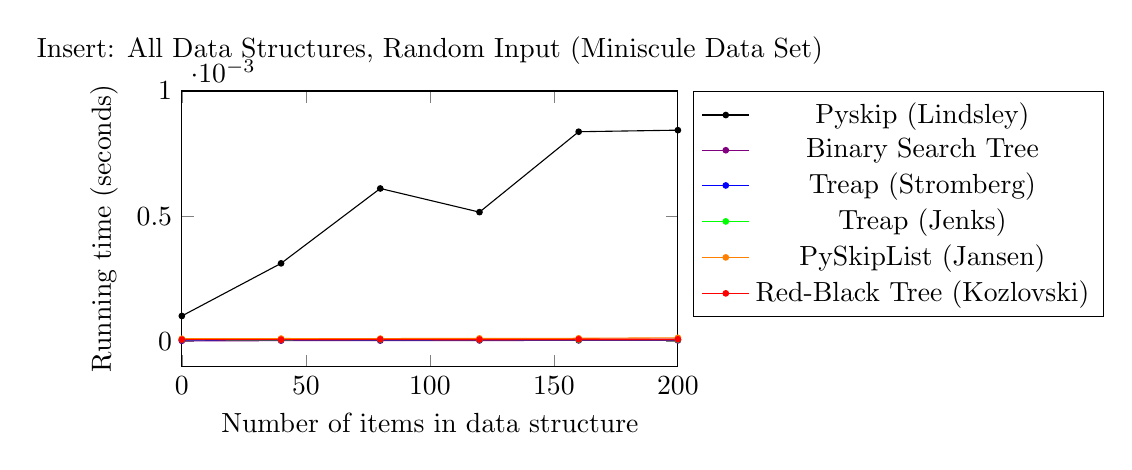
\begin{tikzpicture}
        \begin{axis}[
            title={Insert: All Data Structures, Random Input (Miniscule Data Set)},
            xmin=0, xmax=200,
            ymin=-0.0001, ymax=0.0010,
            xlabel={Number of items in data structure},
            ylabel={Running time (seconds)},
            width=0.65\textwidth,
            height=2in,
            legend pos=outer north east,
        ]
		% Pyskip
		\addplot[
		    color=black, 
		    mark=*,
	    ]
		coordinates {
			(0, 0.00010143585341796358)
			(40, 0.000311535768335931)
			(80, 0.0006105426426629923)
			(120, 0.0005160940570576679)
			(160, 0.0008371770835686271)
			(200, 0.0008434114130393855)
		};
        % BST
		\addplot[
		    color=violet,
		    mark=*,
	    ]
		coordinates {
			(0, 2.1082273572617137e-06)
			(40, 2.8912832328160653e-06)
			(80, 2.9816358338415635e-06)
			(120, 3.6743391083704157e-06)
			(160, 3.7646917093959164e-06)
			(200, 3.794809243071076e-06)
		};
		% Stromberg treap
		\addplot[
		    color=blue,
		    mark=*,
	    ]
        coordinates {
			(0, 5.1500982584523625e-06)
			(40, 6.6559749422101525e-06)
			(80, 6.3849171391350264e-06)
			(120, 6.987267812638698e-06)
			(160, 7.318560683064468e-06)
			(200, 7.288443149391921e-06)
		};
		% Jenks treap
		\addplot[
		    color=green,
		    mark=*,
	    ]
		coordinates {
			(0, 6.776445076911442e-06)
			(40, 6.625857408537605e-06)
			(80, 7.318560683064468e-06)
			(120, 6.9270327452880535e-06)
			(160, 6.776445076911442e-06)
			(200, 7.318560683064468e-06)
		};
		% PySkipList
		\addplot[
		    color=orange,
		    mark=*,
	    ]
         coordinates {
			(0, 1.0511019252634756e-05)
			(40, 1.1294075128187587e-05)
			(80, 1.108325239246033e-05)
			(120, 1.1986778402717224e-05)
			(160, 1.2287953739470447e-05)
			(200, 1.424559342835252e-05)
		};
		% Red-black tree
		\addplot[
		    color=red, 
		    mark=*,
	    ]
         coordinates {
			(0, 6.8366801442620865e-06)
			(40, 6.776445076911442e-06)
			(80, 8.101616558620073e-06)
			(120, 7.348678216742566e-06)
			(160, 8.342556828022651e-06)
			(200, 8.463026962721166e-06)
		};
        \legend{Pyskip (Lindsley), Binary Search Tree, Treap (Stromberg), Treap (Jenks), PySkipList (Jansen), Red-Black Tree (Kozlovski)}
        \end{axis}
    \end{tikzpicture}
    \caption{Average of 10 operations, benchmarked every 40, starting at 0.}
\end{figure}

Clearly Pyskip is too slow for further consideration. In fact, I began with a 105-million-element benchmark that my reference BST implementation handled in about a minute. Pyskip took so long that I eventually had to cancel the benchmark. I had to pare the initial benchmark down to below 1,000 elements to achieve a running time that would not dwarf the rest of my benchmarks combined. With Pyskip eliminated, a graph with larger (but still quite modest) data sets presents a clearer picture of the comparability of the various data structures with random inputs:

\begin{figure}[h]
    \centering
    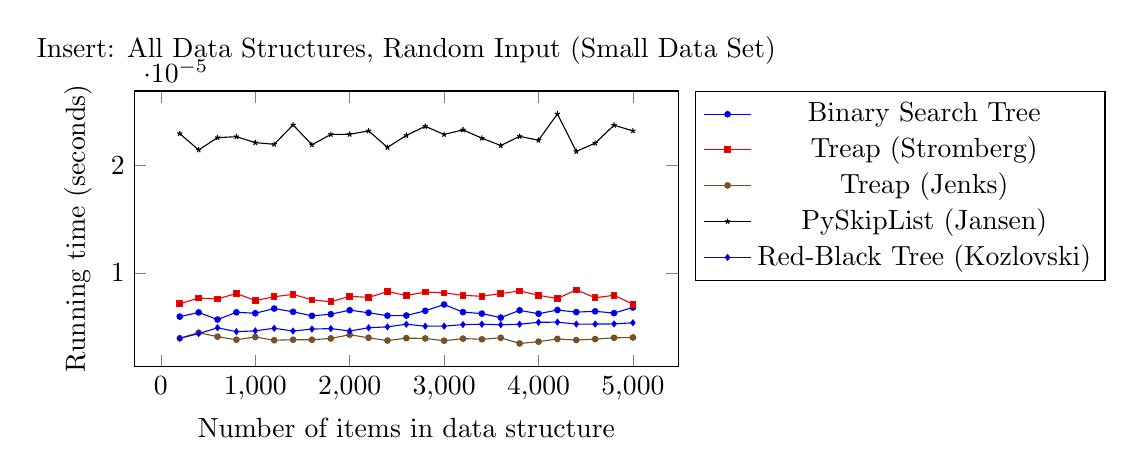
\begin{tikzpicture}
        \begin{axis}[
            xlabel={Number of items in data structure},
            ylabel={Running time (seconds)},
            title={Insert: All Data Structures, Random Input (Small Data Set)},
            width=0.7\textwidth,
            height=2in,
            legend pos=outer north east
        ]
		\addplot coordinates {
			(200, 5.933154134041274e-06)
			(400, 6.324682071845444e-06)
			(600, 5.662096330993905e-06)
			(800, 6.3397408387011465e-06)
			(1000, 6.249388237655751e-06)
			(1200, 6.686092475849392e-06)
			(1400, 6.384917139090618e-06)
			(1600, 6.00844796814215e-06)
			(1800, 6.159035636521537e-06)
			(2000, 6.535504807558823e-06)
			(2200, 6.29456453813404e-06)
			(2400, 6.023506734997852e-06)
			(2600, 6.0385655018535545e-06)
			(2800, 6.475269740136014e-06)
			(3000, 7.062561646886678e-06)
			(3200, 6.354799605468031e-06)
			(3400, 6.219270703944346e-06)
			(3600, 5.842801532995878e-06)
			(3800, 6.520446040703121e-06)
			(4000, 6.204211937088644e-06)
			(4200, 6.550563574414525e-06)
			(4400, 6.354799605468031e-06)
			(4600, 6.430093439568907e-06)
			(4800, 6.264447004422635e-06)
			(5000, 6.7915038437504904e-06)
		};
		\addplot coordinates {
			(200, 7.137855480987554e-06)
			(400, 7.664912320315409e-06)
			(600, 7.5896184861257154e-06)
			(800, 8.086557791830984e-06)
			(1000, 7.439030817746328e-06)
			(1200, 7.785382454983391e-06)
			(1400, 8.01126395764129e-06)
			(1600, 7.499265885169137e-06)
			(1800, 7.318560683078346e-06)
			(2000, 7.830558755550498e-06)
			(2200, 7.7251473876494e-06)
			(2400, 8.267262993832958e-06)
			(2600, 7.905852589740191e-06)
			(2800, 8.222086693265851e-06)
			(3000, 8.146792859164976e-06)
			(3200, 7.920911356507076e-06)
			(3400, 7.830558755550498e-06)
			(3600, 8.086557791742166e-06)
			(3800, 8.327498061166948e-06)
			(4000, 7.920911356595894e-06)
			(4200, 7.61973601983712e-06)
			(4400, 8.43290942897923e-06)
			(4600, 7.695029853937996e-06)
			(4800, 7.920911356595894e-06)
			(5000, 7.092679180509265e-06)
		};
		\addplot coordinates {
			(200, 3.915279377775249e-06)
			(400, 4.4423362171031044e-06)
			(600, 4.0658670461546365e-06)
			(800, 3.7797504762515643e-06)
			(1000, 4.035749512443232e-06)
			(1200, 3.7345741756844575e-06)
			(1400, 3.7797504761627465e-06)
			(1600, 3.7797504762515643e-06)
			(1800, 3.900220611008365e-06)
			(2000, 4.246572248156611e-06)
			(2200, 3.960455678342356e-06)
			(2400, 3.7044566420618706e-06)
			(2600, 3.930338144630951e-06)
			(2800, 3.900220610919547e-06)
			(3000, 3.6893978752061685e-06)
			(3200, 3.885161844152662e-06)
			(3400, 3.824926776729854e-06)
			(3600, 3.960455678342356e-06)
			(3800, 3.433398838925683e-06)
			(4000, 3.5990452741607727e-06)
			(4200, 3.855044310441258e-06)
			(4400, 3.7496329425401596e-06)
			(4600, 3.839985543585556e-06)
			(4800, 3.960455678253538e-06)
			(5000, 3.990573211964943e-06)
		};
		\addplot coordinates {
			(200, 2.2994736960946228e-05)
			(400, 2.147380151038547e-05)
			(600, 2.261826778999776e-05)
			(800, 2.2708620391043154e-05)
			(1000, 2.2151446018092714e-05)
			(1200, 2.2000858349713327e-05)
			(1400, 2.3807910370177156e-05)
			(1600, 2.195568204914622e-05)
			(1800, 2.2919443126845353e-05)
			(2000, 2.2934501893612236e-05)
			(2200, 2.3250735997226712e-05)
			(2400, 2.1714741779810254e-05)
			(2600, 2.2829090525799955e-05)
			(2800, 2.367238146865347e-05)
			(3000, 2.2919443126845353e-05)
			(3200, 2.334108859827211e-05)
			(3400, 2.257309148951947e-05)
			(3600, 2.1880388215045343e-05)
			(3800, 2.273873792475456e-05)
			(4000, 2.2377327520661795e-05)
			(4200, 2.483190651512146e-05)
			(4400, 2.1338272608861786e-05)
			(4600, 2.2106269717614425e-05)
			(4800, 2.3777792836554566e-05)
			(5000, 2.3250735997226712e-05)
		};
		\addplot coordinates {
			(200, 3.915279377775249e-06)
			(400, 4.351983616057708e-06)
			(600, 4.894099222241266e-06)
			(800, 4.5326888180596825e-06)
			(1000, 4.607982652338194e-06)
			(1200, 4.848922921762977e-06)
			(1400, 4.592923885482492e-06)
			(1600, 4.773629087484465e-06)
			(1800, 4.8188053880515724e-06)
			(2000, 4.592923885393674e-06)
			(2200, 4.894099222241266e-06)
			(2400, 4.984451823286662e-06)
			(2600, 5.225392092622627e-06)
			(2800, 5.044686890620653e-06)
			(3000, 5.044686890620653e-06)
			(3200, 5.1952745590000404e-06)
			(3400, 5.225392092622627e-06)
			(3600, 5.180215792144338e-06)
			(3800, 5.225392092711445e-06)
			(4000, 5.406097294713419e-06)
			(4200, 5.421156061480304e-06)
			(4400, 5.2404508594783294e-06)
			(4600, 5.2404508594783294e-06)
			(4800, 5.2555096263340316e-06)
			(5000, 5.360920994146312e-06)
		};
        \legend{Binary Search Tree, Treap (Stromberg), Treap (Jenks), PySkipList (Jansen), Red-Black Tree (Kozlovski)}
        \end{axis}
    \end{tikzpicture}
    \caption{Average of 20 operations, benchmarked every 200, starting at 200.}
\end{figure}

Based on these benchmark results, the only remaining skiplist implementation is again the clear outlier, but in this case, the difference is much less pronounced. Compared to the binary search tree reference implementation, PySkipList benchmarks on insertion at only about 2.5 times slower, and this, of course, is under ideal conditions for a binary search tree.

Comparing the Stromberg and Jenks treaps, the latter appears to be two or three times faster in this particular benchmark. Interestingly, both are comparable or superior to the binary search tree, and the Jenks treap is faster than both the binary search tree and the Kozlovski red-black tree! Because the treaps provide such interesting counterpoints, both to one another and to the deterministic data structures used here, I will keep both. Thus, the data structures are finalized.

\section{Choosing Inputs \& Benchmarks}
The remainder of this paper examines the above implementations' performance on the insert, search, and delete operations with large data sets ($10^6$ or larger). The two essential cases are randomized input and ordered input (the binary search tree's worst-case input). Beyond these, I will add as many more novel configurations as space allows.

The SIDGraphSet and SIDBenchmark classes in sidgraphset.py perform the first two benchmark sets. Their sequence, in short, is to perform insertions up to each data point, benchmark a number of searches on selected elements that have already been inserted, benchmark a number of insertions, and repeat. Once all insertions are complete, the sequence continues with deletions: SIDBenchmark will delete elements until it reaches the last graph point plus the sample size, benchmark deletions down to the graph plot point, and repeat this cycle until it benchmarks the first plot point.

The SIDBenchmark class implements this benchmark sequence, and the SIDGraphSet class collates the three plots (search, insert, and delete) of a set of SIDBenchmarks into three final graphs. The full pseudocode for the SIDBenchmark sequence is below, updated for presentation here, along with opening notes copied from the source comments.

\begin{Verbatim}
Instantiates a Plot containing the results of a full suite of search, insert, and
delete benchmarks. Runs these benchmarks immediately and synchronously. Saves the
results as instance variables. Note that this benchmark differs substantially from
BenchmarkPlot, even though its interface is similar!

The benchmark accepts 3 sample sets and maintain 3 indices: one apiece for search,
index, and delete. The data structure on which search, insert, and delete are called is
presumed to be empty prior to this benchmark; the plot points count from 0 elements.
Each index starts at 0.

The sample sets should have the following minimum sizes:
    len(search_samples) >= the number of searches requested 
        (likely bm_length times some integer)
    len(insert_samples) >= stop
    len(delete_samples) >= stop

0. Set next_benchmark as bm_start.
1. Call insert on the items in insert_samples with indices [0, bm_start).
2. While insert_index < stop:
    a. Set last_benchmark as next_benchmark.
    b. Set next_benchmark as min(next_benchmark + bm_interval, stop).
    c. Benchmark: time bm_length searches on items in search_samples[search_index],
       incrementing search_index each time. Divide the total time by bm_length 
       and save (data structure size, time) as a plot point for insert.
    d. Benchmark: time bm_length inserts on items in insert_samples[insert_index],
       incrementing insert_index each time. Divide the total time by bm_length 
       and save (data structure size before timed insertions, time) as a plot point
       for insert.
    e. Insert subsequent items from insert_samples, incrementing insert_index, until
       insert_index == next_benchmark. These insertions are not timed.
3. Set next_benchmark = last_benchmark + bm_length.
4. While data structure size > bm_start:
    a. Delete items from delete_samples[delete_index], decrementing delete_index,
       until data structure size == next_benchmark.
    b. Benchmark: time bm_length deletions on items in delete_samples[delete_index],
       decrementing delete_index each time. Divide the total time by bm_length 
       and save (data structure size after timed deletions, time) as a plot point
       for delete.
    c. Decrease next_benchmark by bm_interval.
\end{Verbatim}

\section{Benchmarks: Randomized Inputs}
Random inputs are, of course, the best-case scenario for binary search tree insertions. The other data structures should perform well on randomized inputs, too. As a result, this benchmark serves as a useful baseline for later comparisons. The average-case asymptotic performance for all four data structures is $O(\log n)$, and I expect this performance from all five implementations with this input set.

\begin{figure}[h]
    \centering
    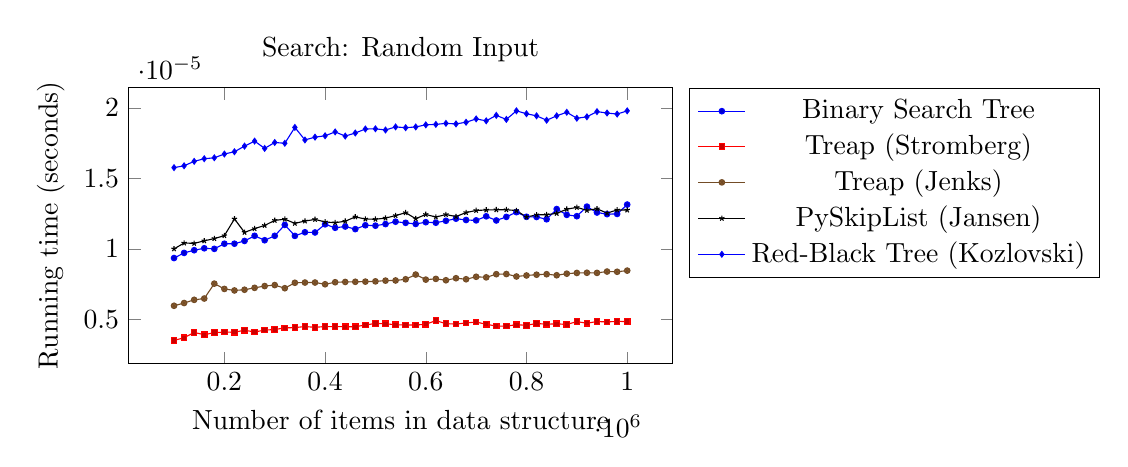
\begin{tikzpicture}
        \begin{axis}[
            xlabel={Number of items in data structure},
            ylabel={Running time (seconds)},
            title={Search: Random Input},
            width=0.7\textwidth,
            height=2in,
            legend pos=outer north east
        ]
		\addplot coordinates {
			(100000, 9.348482452771942e-06)
			(120000, 9.712001084231203e-06)
			(140000, 9.903548598405254e-06)
			(160000, 1.0040884551964058e-05)
			(180000, 9.999322355492279e-06)
			(200000, 1.0364045688298518e-05)
			(220000, 1.0365852740319204e-05)
			(240000, 1.056041200786062e-05)
			(260000, 1.0923629463983175e-05)
			(280000, 1.061070828909827e-05)
			(300000, 1.0922424762636051e-05)
			(320000, 1.1699758306792152e-05)
			(340000, 1.0920015359942248e-05)
			(360000, 1.1177821448201452e-05)
			(380000, 1.1161859155353503e-05)
			(400000, 1.1739513451243244e-05)
			(420000, 1.149556142847441e-05)
			(440000, 1.1583203451469792e-05)
			(460000, 1.1399486496050493e-05)
			(480000, 1.167235135114808e-05)
			(500000, 1.1643137343482656e-05)
			(520000, 1.1755776919427418e-05)
			(540000, 1.1924736283345893e-05)
			(560000, 1.1845527169780823e-05)
			(580000, 1.1765715705540636e-05)
			(600000, 1.1890101119619524e-05)
			(620000, 1.1854261254545584e-05)
			(640000, 1.198979015608348e-05)
			(660000, 1.2140980175133542e-05)
			(680000, 1.2046109944057193e-05)
			(700000, 1.2019004163748903e-05)
			(720000, 1.230753013635688e-05)
			(740000, 1.2013583007687955e-05)
			(760000, 1.2265967939883993e-05)
			(780000, 1.2603585492383828e-05)
			(800000, 1.2275304375325646e-05)
			(820000, 1.226084795916016e-05)
			(840000, 1.2097912101978636e-05)
			(860000, 1.2821034085519044e-05)
			(880000, 1.2410532101524653e-05)
			(900000, 1.2317167747132985e-05)
			(920000, 1.2995113430161353e-05)
			(940000, 1.2576178536738426e-05)
			(960000, 1.2460828382764078e-05)
			(980000, 1.2476790675611581e-05)
			(1000000, 1.3140581117811579e-05)
		};
		\addplot coordinates {
			(100000, 3.506885621135325e-06)
			(120000, 3.692108453240195e-06)
			(140000, 4.071890552882706e-06)
			(160000, 3.908352345028731e-06)
			(180000, 4.058036487393224e-06)
			(200000, 4.092671651118707e-06)
			(220000, 4.085443443038628e-06)
			(240000, 4.2294052540015055e-06)
			(260000, 4.1044174892519434e-06)
			(280000, 4.234826410066006e-06)
			(300000, 4.278496833894252e-06)
			(320000, 4.394449338544604e-06)
			(340000, 4.414326910769262e-06)
			(360000, 4.490524270970297e-06)
			(380000, 4.433602132323245e-06)
			(400000, 4.489319569621841e-06)
			(420000, 4.485705465580025e-06)
			(440000, 4.475164328795245e-06)
			(460000, 4.474863153458131e-06)
			(480000, 4.600453268881921e-06)
			(500000, 4.708274039437299e-06)
			(520000, 4.6896011685610975e-06)
			(540000, 4.612500282352272e-06)
			(560000, 4.603163846908842e-06)
			(580000, 4.598345041529228e-06)
			(600000, 4.650147199448895e-06)
			(620000, 4.910061515062125e-06)
			(640000, 4.693215272602913e-06)
			(660000, 4.664603615609053e-06)
			(680000, 4.745318605856142e-06)
			(700000, 4.807963075904809e-06)
			(720000, 4.6525566021387025e-06)
			(740000, 4.520039453971947e-06)
			(760000, 4.521545330653964e-06)
			(780000, 4.618222613750334e-06)
			(800000, 4.57786511862679e-06)
			(820000, 4.707972864096632e-06)
			(840000, 4.652857777472264e-06)
			(860000, 4.6844811878372635e-06)
			(880000, 4.635991958615193e-06)
			(900000, 4.8386829602549145e-06)
			(920000, 4.7254410336350365e-06)
			(940000, 4.841694713626054e-06)
			(960000, 4.8185042126931425e-06)
			(980000, 4.8537417270893e-06)
			(1000000, 4.846513519005669e-06)
		};
		\addplot coordinates {
			(100000, 5.962368141673835e-06)
			(120000, 6.157830935222819e-06)
			(140000, 6.383712437788347e-06)
			(160000, 6.475570915497997e-06)
			(180000, 7.533298698170654e-06)
			(200000, 7.1580342285813e-06)
			(220000, 7.049912282681703e-06)
			(240000, 7.099907388585791e-06)
			(260000, 7.234532764115898e-06)
			(280000, 7.3604240548732496e-06)
			(300000, 7.429393206990653e-06)
			(320000, 7.207728159137616e-06)
			(340000, 7.59383494085597e-06)
			(360000, 7.609797233698146e-06)
			(380000, 7.6113031103872685e-06)
			(400000, 7.488423572993952e-06)
			(420000, 7.632084208623268e-06)
			(440000, 7.652564131525707e-06)
			(460000, 7.664008794321831e-06)
			(480000, 7.676055807785075e-06)
			(500000, 7.693222801982813e-06)
			(520000, 7.746832011925164e-06)
			(540000, 7.757373148713497e-06)
			(560000, 7.841401067672393e-06)
			(580000, 8.17691039281243e-06)
			(600000, 7.817005865391025e-06)
			(620000, 7.870012724659148e-06)
			(640000, 7.773034266229218e-06)
			(660000, 7.916092551184307e-06)
			(680000, 7.844713996377096e-06)
			(700000, 8.019094516356517e-06)
			(720000, 7.978737021232973e-06)
			(740000, 8.202510296428045e-06)
			(760000, 8.213051433216378e-06)
			(780000, 8.039875614585413e-06)
			(800000, 8.11245887074108e-06)
			(820000, 8.166068080683431e-06)
			(840000, 8.201004419746028e-06)
			(860000, 8.127818812923238e-06)
			(880000, 8.238048986171976e-06)
			(900000, 8.291357020780765e-06)
			(920000, 8.303404034236906e-06)
			(940000, 8.295874650812607e-06)
			(960000, 8.388937829877818e-06)
			(980000, 8.374481413710555e-06)
			(1000000, 8.456099929972539e-06)
		};
		\addplot coordinates {
			(100000, 9.996611777467024e-06)
			(120000, 1.0412233742172817e-05)
			(140000, 1.0390549117929027e-05)
			(160000, 1.05670378652718e-05)
			(180000, 1.0729672547114432e-05)
			(200000, 1.093477295144396e-05)
			(220000, 1.2122006128919338e-05)
			(240000, 1.1169388538775138e-05)
			(260000, 1.143291695842663e-05)
			(280000, 1.166211138969686e-05)
			(300000, 1.2018100637746443e-05)
			(320000, 1.2103634433373145e-05)
			(340000, 1.1808783778690212e-05)
			(360000, 1.1971719635880618e-05)
			(380000, 1.2087370965190303e-05)
			(400000, 1.1907268113816372e-05)
			(420000, 1.1854261254541144e-05)
			(440000, 1.1958769096409583e-05)
			(460000, 1.226657029056355e-05)
			(480000, 1.211266969347946e-05)
			(500000, 1.2098815627993532e-05)
			(520000, 1.2180132968921954e-05)
			(540000, 1.2358729943599655e-05)
			(560000, 1.2564733873944079e-05)
			(580000, 1.2140678999799092e-05)
			(600000, 1.2439746109194517e-05)
			(620000, 1.2255727978427445e-05)
			(640000, 1.2433421427118674e-05)
			(660000, 1.2289459616155795e-05)
			(680000, 1.2574070309383956e-05)
			(700000, 1.2722248575073536e-05)
			(720000, 1.2755679037439905e-05)
			(740000, 1.277254485630408e-05)
			(760000, 1.277646013568301e-05)
			(780000, 1.2714719191649238e-05)
			(800000, 1.2255426803093883e-05)
			(820000, 1.2411435627541324e-05)
			(840000, 1.2423181465678112e-05)
			(860000, 1.251564229406199e-05)
			(880000, 1.2811095299412045e-05)
			(900000, 1.2941504220222555e-05)
			(920000, 1.2730380309164957e-05)
			(940000, 1.2839405781051027e-05)
			(960000, 1.2536122216957324e-05)
			(980000, 1.2758088440136816e-05)
			(1000000, 1.2750257881378957e-05)
		};
		\addplot coordinates {
			(100000, 1.5759903021518086e-05)
			(120000, 1.5891817819039033e-05)
			(140000, 1.6205943695268842e-05)
			(160000, 1.6391768878065704e-05)
			(180000, 1.6457726276797758e-05)
			(200000, 1.6726374677176636e-05)
			(220000, 1.688720230700369e-05)
			(240000, 1.7285958452845307e-05)
			(260000, 1.7643152402229136e-05)
			(280000, 1.7123624946350446e-05)
			(300000, 1.754587276846564e-05)
			(320000, 1.7487444753129467e-05)
			(340000, 1.8613539337252406e-05)
			(360000, 1.7723867392504644e-05)
			(380000, 1.7923245465425453e-05)
			(400000, 1.8018416871854015e-05)
			(420000, 1.8293389954294525e-05)
			(440000, 1.7998840474973577e-05)
			(460000, 1.8215686717411472e-05)
			(480000, 1.849999623530607e-05)
			(500000, 1.8514452651487544e-05)
			(520000, 1.843042473251444e-05)
			(540000, 1.8648475676315003e-05)
			(560000, 1.8593059414371284e-05)
			(580000, 1.8646969799647195e-05)
			(600000, 1.879575041598969e-05)
			(620000, 1.882827735235537e-05)
			(640000, 1.8899957082510355e-05)
			(660000, 1.8861105464083038e-05)
			(680000, 1.8979166196089635e-05)
			(700000, 1.9215890010769952e-05)
			(720000, 1.90791564078836e-05)
			(740000, 1.9467973767632428e-05)
			(760000, 1.918125484704092e-05)
			(780000, 1.9789327851952976e-05)
			(800000, 1.958061334357808e-05)
			(820000, 1.9435446831238323e-05)
			(840000, 1.912222448103762e-05)
			(860000, 1.94348444805712e-05)
			(880000, 1.968963881546415e-05)
			(900000, 1.9263475713955812e-05)
			(920000, 1.9363767101111762e-05)
			(940000, 1.9732405713284606e-05)
			(960000, 1.963452372885399e-05)
			(980000, 1.9559832245334975e-05)
			(1000000, 1.978782197525675e-05)
		};
        \legend{Binary Search Tree, Treap (Stromberg), Treap (Jenks), PySkipList (Jansen), Red-Black Tree (Kozlovski)}
        \end{axis}
    \end{tikzpicture}
    \caption{Average of 1000 operations, benchmarked every 20000, starting at 100000.}
\end{figure}

Search is perhaps the most interesting graph, because, surprisingly, the graphs of the five plots all curve to plausibly match the graph of $c \cdot \log n$ for various constant multiples $c$. Clearly, all five do in fact work in logarithmic time! Both treaps are the clear winners for search. PySkipList, the slowest implementation in the small data set benchmark above, is neck-and-neck with the binary search tree. Finally, the red-black tree, the second-fastest on insertion in the small data set benchmark, is the standout slowest here.

\begin{figure}[ht]
    \centering
    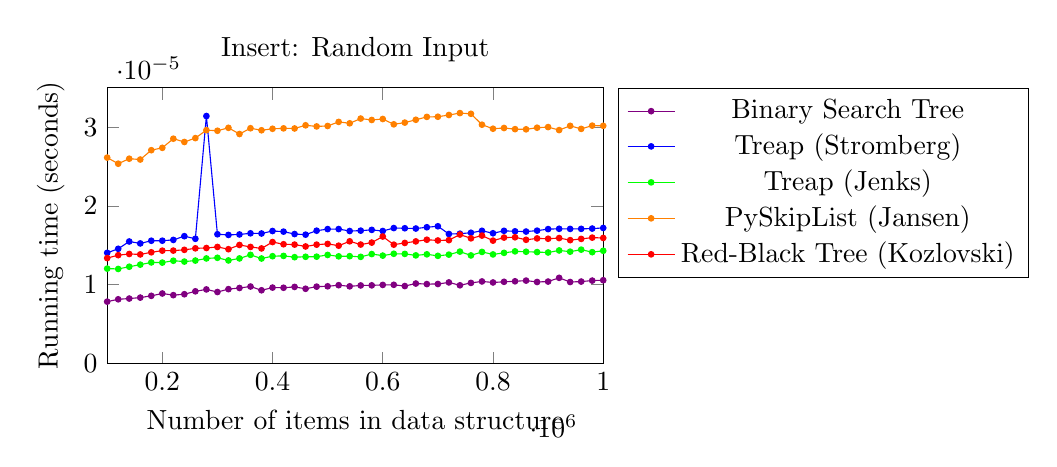
\begin{tikzpicture}
        \begin{axis}[
            title={Insert: Random Input},
            xmin=100000, xmax=1000000,
            ymin=0, ymax=0.000035,
            xlabel={Number of items in data structure},
            ylabel={Running time (seconds)},
            width=0.65\textwidth,
            height=2in,
            legend pos=outer north east,
        ]
        % BST
		\addplot[
		    color=violet,
		    mark=*,
	    ]
	    coordinates {
			(100000, 7.8380881389623e-06)
			(120000, 8.138058774366962e-06)
			(140000, 8.232025479433469e-06)
			(160000, 8.352495614134203e-06)
			(180000, 8.577473590687613e-06)
			(200000, 8.872625420704328e-06)
			(220000, 8.664513263008989e-06)
			(240000, 8.77986341698489e-06)
			(260000, 9.150911431862863e-06)
			(280000, 9.39155052592744e-06)
			(300000, 9.062365882857915e-06)
			(320000, 9.42648686499048e-06)
			(340000, 9.574966306009181e-06)
			(360000, 9.759586787438046e-06)
			(380000, 9.281621528013151e-06)
			(400000, 9.62435906123682e-06)
			(420000, 9.6047826643475e-06)
			(440000, 9.709892856874625e-06)
			(460000, 9.47557844488145e-06)
			(480000, 9.744829195937221e-06)
			(500000, 9.790005496450149e-06)
			(520000, 9.928847326691859e-06)
			(540000, 9.785186691061653e-06)
			(560000, 9.89571803965017e-06)
			(580000, 9.909270929803426e-06)
			(600000, 9.964687191765797e-06)
			(620000, 9.978541257257057e-06)
			(640000, 9.820725380798478e-06)
			(660000, 1.013846536107188e-05)
			(680000, 1.006919503361825e-05)
			(700000, 1.0080639696415261e-05)
			(720000, 1.028122247069252e-05)
			(740000, 9.915896787211054e-06)
			(760000, 1.022128857867699e-05)
			(780000, 1.0406511410780084e-05)
			(800000, 1.0275801314630683e-05)
			(820000, 1.0359226882910022e-05)
			(840000, 1.0425184281659838e-05)
			(860000, 1.051282630465522e-05)
			(880000, 1.0337241083327343e-05)
			(900000, 1.0390549117932579e-05)
			(920000, 1.0863695571970311e-05)
			(940000, 1.0332422277938847e-05)
			(960000, 1.0390247942595465e-05)
			(980000, 1.0515235707346804e-05)
			(1000000, 1.0559508481851055e-05)
		};
		% Stromberg treap
		\addplot[
		    color=blue,
		    mark=*,
	    ]
		coordinates {
			(100000, 1.4039589498015203e-05)
			(120000, 1.4554298148524935e-05)
			(140000, 1.5481918185720645e-05)
			(160000, 1.5235255584919117e-05)
			(180000, 1.557678841679433e-05)
			(200000, 1.55837154495444e-05)
			(220000, 1.5681898609322787e-05)
			(240000, 1.6155647414031192e-05)
			(260000, 1.5826763946300558e-05)
			(280000, 3.141981583128129e-05)
			(300000, 1.639959943680225e-05)
			(320000, 1.6317679745203152e-05)
			(340000, 1.637671011120645e-05)
			(360000, 1.652067192217643e-05)
			(380000, 1.6497782596584187e-05)
			(400000, 1.681220964815111e-05)
			(420000, 1.67354099372794e-05)
			(440000, 1.6428211093792554e-05)
			(460000, 1.6350809032246616e-05)
			(480000, 1.6852567143278206e-05)
			(500000, 1.705646284625928e-05)
			(520000, 1.7060980476305332e-05)
			(540000, 1.6811908472813997e-05)
			(560000, 1.6859795351358286e-05)
			(580000, 1.6958580861818008e-05)
			(600000, 1.68131131741589e-05)
			(620000, 1.718867881908892e-05)
			(640000, 1.716277774013264e-05)
			(660000, 1.7128744927077833e-05)
			(680000, 1.7291680784261132e-05)
			(700000, 1.7417270899684923e-05)
			(720000, 1.6434836951198405e-05)
			(740000, 1.6472483868298582e-05)
			(760000, 1.6592954002994986e-05)
			(780000, 1.6838110727114496e-05)
			(800000, 1.6529707182279198e-05)
			(820000, 1.6836303675091813e-05)
			(840000, 1.6773358029709585e-05)
			(860000, 1.6743541671374372e-05)
			(880000, 1.6861000052706744e-05)
			(900000, 1.7055258144914375e-05)
			(920000, 1.7094109763348797e-05)
			(940000, 1.7082062749885552e-05)
			(960000, 1.7088989782628518e-05)
			(980000, 1.7123022595683325e-05)
			(1000000, 1.7201629358574167e-05)
		};
		% Jenks treap
		\addplot[
		    color=green,
		    mark=*,
	    ]
		coordinates {
			(100000, 1.2039484086649565e-05)
			(120000, 1.1992500734116617e-05)
			(140000, 1.2276509076670549e-05)
			(160000, 1.253943514565492e-05)
			(180000, 1.2821636436193273e-05)
			(200000, 1.2798144759926799e-05)
			(220000, 1.3037579152637591e-05)
			(240000, 1.2929457206752204e-05)
			(260000, 1.3058661426214257e-05)
			(280000, 1.3328213352608031e-05)
			(300000, 1.3411337745552032e-05)
			(320000, 1.3075828420411994e-05)
			(340000, 1.3330321579964276e-05)
			(360000, 1.3785096338459368e-05)
			(380000, 1.3319780443175943e-05)
			(400000, 1.361252287050263e-05)
			(420000, 1.3652579190285507e-05)
			(440000, 1.3488438631760857e-05)
			(460000, 1.3539337263672734e-05)
			(480000, 1.3554697205847788e-05)
			(500000, 1.3771844623647667e-05)
			(520000, 1.3595054700971332e-05)
			(540000, 1.3615835799207333e-05)
			(560000, 1.3529097302217963e-05)
			(580000, 1.388327949824486e-05)
			(600000, 1.3688419055363e-05)
			(620000, 1.3920625239997263e-05)
			(640000, 1.3905867648503546e-05)
			(660000, 1.3716729537023298e-05)
			(680000, 1.3850451386531403e-05)
			(700000, 1.3657397995686438e-05)
			(720000, 1.3813105644771895e-05)
			(740000, 1.4197706549808232e-05)
			(760000, 1.3710706030295228e-05)
			(780000, 1.4157047879351126e-05)
			(800000, 1.3839307899075948e-05)
			(820000, 1.4037180095328949e-05)
			(840000, 1.4226619382128547e-05)
			(860000, 1.417963602960981e-05)
			(880000, 1.4135062079759564e-05)
			(900000, 1.4083561097180563e-05)
			(920000, 1.4344680114149355e-05)
			(940000, 1.4188370114382564e-05)
			(960000, 1.4443766799942636e-05)
			(980000, 1.4126327994986809e-05)
			(1000000, 1.4301913216314688e-05)
		};
		% PySkipList
		\addplot[
		    color=orange,
		    mark=*,
	    ]
         coordinates {
			(100000, 2.6140513353368533e-05)
			(120000, 2.5363480984538e-05)
			(140000, 2.600137034778527e-05)
			(160000, 2.5893850752552794e-05)
			(180000, 2.7081987456057278e-05)
			(200000, 2.7381355740786263e-05)
			(220000, 2.854298901462471e-05)
			(240000, 2.8125861173222688e-05)
			(260000, 2.8617680498143726e-05)
			(280000, 2.9629629629624788e-05)
			(300000, 2.9552528743408856e-05)
			(320000, 2.9923576758292826e-05)
			(340000, 2.9136003252688168e-05)
			(360000, 2.987147342503249e-05)
			(380000, 2.9612161460093488e-05)
			(400000, 2.9803106623589314e-05)
			(420000, 2.9854607606182527e-05)
			(440000, 2.9842259417378614e-05)
			(460000, 3.0244328491932037e-05)
			(480000, 3.0103679609680967e-05)
			(500000, 3.0158192345624e-05)
			(520000, 3.0678020976850465e-05)
			(540000, 3.0496713424142286e-05)
			(560000, 3.11017746756761e-05)
			(580000, 3.092167182428796e-05)
			(600000, 3.104515371236971e-05)
			(620000, 3.0368412730680915e-05)
			(640000, 3.0586162499147915e-05)
			(660000, 3.094666937724355e-05)
			(680000, 3.1314103288082154e-05)
			(700000, 3.133096910693211e-05)
			(720000, 3.155414003147427e-05)
			(740000, 3.1796586177563315e-05)
			(760000, 3.170683592720991e-05)
			(780000, 3.0321128202800196e-05)
			(800000, 2.98082266043167e-05)
			(820000, 2.9901590958715472e-05)
			(840000, 2.9756424446404138e-05)
			(860000, 2.9732631594797e-05)
			(880000, 2.9939539051156318e-05)
			(900000, 3.0018446989373615e-05)
			(920000, 2.963595431170063e-05)
			(940000, 3.0176865216503756e-05)
			(960000, 2.9790758434799614e-05)
			(980000, 3.0203970996808493e-05)
			(1000000, 3.0180780495882685e-05)
		};
		% Red-black tree
		\addplot[
		    color=red, 
		    mark=*,
	    ]
	    coordinates {
			(100000, 1.3373088477777627e-05)
			(120000, 1.3744437668009369e-05)
			(140000, 1.3894422985714527e-05)
			(160000, 1.3836597321045474e-05)
			(180000, 1.4110064526818178e-05)
			(200000, 1.4316670807829724e-05)
			(220000, 1.4324501366587583e-05)
			(240000, 1.4420576298988409e-05)
			(260000, 1.4613930865209567e-05)
			(280000, 1.4654890711000235e-05)
			(300000, 1.4788010209827007e-05)
			(320000, 1.4504303042627952e-05)
			(340000, 1.5042202194081256e-05)
			(360000, 1.4789817261885218e-05)
			(380000, 1.4598872098360971e-05)
			(400000, 1.541053963092054e-05)
			(420000, 1.513014539239066e-05)
			(440000, 1.5087980845237326e-05)
			(460000, 1.4850955855251868e-05)
			(480000, 1.5080451461813027e-05)
			(500000, 1.5176526394242274e-05)
			(520000, 1.4948837839654062e-05)
			(540000, 1.5505108686653557e-05)
			(560000, 1.509249847529759e-05)
			(580000, 1.5340666952795345e-05)
			(600000, 1.6112278165536507e-05)
			(620000, 1.5078644409811659e-05)
			(640000, 1.5295791827611538e-05)
			(660000, 1.549245932250187e-05)
			(680000, 1.5706896162271278e-05)
			(700000, 1.561232710653826e-05)
			(720000, 1.5653286952357347e-05)
			(740000, 1.6362554870397615e-05)
			(760000, 1.5882180208251385e-05)
			(780000, 1.6232447124906456e-05)
			(800000, 1.5591847183628714e-05)
			(820000, 1.5977050439346384e-05)
			(840000, 1.6017709109803492e-05)
			(860000, 1.569755972684561e-05)
			(880000, 1.587555435085619e-05)
			(900000, 1.5830378050367245e-05)
			(920000, 1.5918923599372193e-05)
			(940000, 1.5653588127662488e-05)
			(960000, 1.5809898127429277e-05)
			(980000, 1.597223163395256e-05)
			(1000000, 1.593036826213279e-05)
		};
        \legend{Binary Search Tree, Treap (Stromberg), Treap (Jenks), PySkipList (Jansen), Red-Black Tree (Kozlovski)}
        \end{axis}
    \end{tikzpicture}
    \caption{Average of 1000 operations, benchmarked every 20000, starting at 100000.}
    \label{fig:random_insert}
\end{figure}

Next up is insertion. Here, the logarithmic graph is faintly visible at best. The most telling is perhaps the binary search tree, whose running time approximately doubles from $10^5$ elements to $10^6$ elements, in keeping with a logarithmic rate of growth.  In comparison to the small data set insertion benchmark, almost everything is the same: the treaps and red-black tree are all tightly grouped, and PySkipList takes about twice as long as the rest. However, in this best-case input for the binary search tree, it does indeed pull ahead of the pack.

\begin{figure}[h]
    \centering
    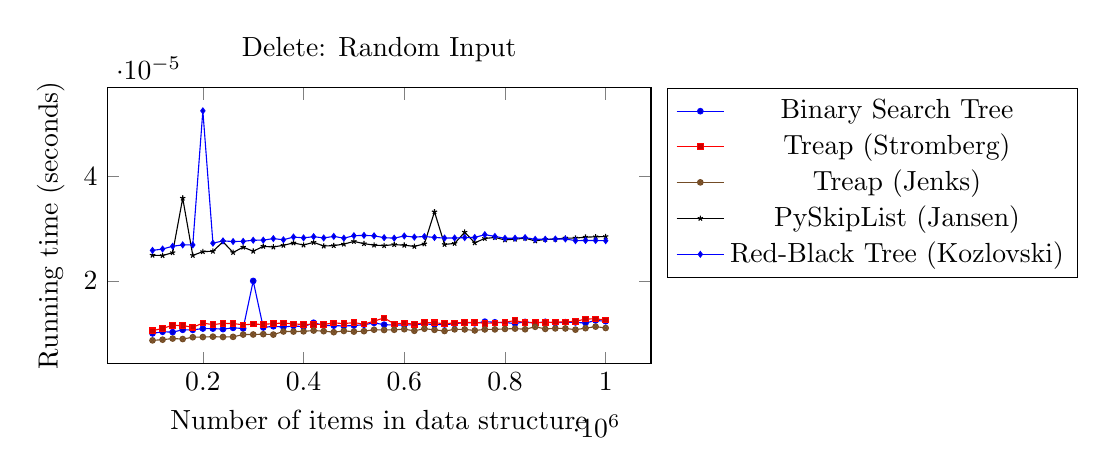
\begin{tikzpicture}
        \begin{axis}[
            xlabel={Number of items in data structure},
            ylabel={Running time (seconds)},
            title={Delete: Random Input},
            width=0.7\textwidth,
            height=2in,
            legend pos=outer north east
        ]
		\addplot coordinates {
			(1000000, 1.2300301928275913e-05)
			(980000, 1.2457515454059375e-05)
			(960000, 1.1958166745726472e-05)
			(940000, 1.2082552159803583e-05)
			(920000, 1.21256202329576e-05)
			(900000, 1.1965997304480779e-05)
			(880000, 1.2193987034400778e-05)
			(860000, 1.1927446861376367e-05)
			(840000, 1.2181638845595088e-05)
			(820000, 1.1870825898068205e-05)
			(800000, 1.2046712294731422e-05)
			(780000, 1.2106345011407172e-05)
			(760000, 1.2221092814709068e-05)
			(740000, 1.1908773990498388e-05)
			(720000, 1.2090985069233895e-05)
			(700000, 1.1793423836522265e-05)
			(680000, 1.1666629019750019e-05)
			(660000, 1.1665725493740452e-05)
			(640000, 1.180667555133752e-05)
			(620000, 1.1618742141209282e-05)
			(600000, 1.1594648114265028e-05)
			(580000, 1.158109522411266e-05)
			(560000, 1.1640125590112405e-05)
			(540000, 1.1984369000021644e-05)
			(520000, 1.1635909135399914e-05)
			(500000, 1.1477792083606885e-05)
			(480000, 1.1401293548068736e-05)
			(460000, 1.1464239193450964e-05)
			(440000, 1.1498573181842886e-05)
			(420000, 1.201358300768618e-05)
			(400000, 1.1264559945185938e-05)
			(380000, 1.1401293548072289e-05)
			(360000, 1.1195590793068533e-05)
			(340000, 1.1337745552015832e-05)
			(320000, 1.1104635841370225e-05)
			(300000, 2.00251481406184e-05)
			(280000, 1.0921220061291591e-05)
			(260000, 1.103145023454033e-05)
			(240000, 1.0792015841822433e-05)
			(220000, 1.0889596650933697e-05)
			(200000, 1.0902547190411837e-05)
			(180000, 1.0643536400806396e-05)
			(160000, 1.0664317499042397e-05)
			(140000, 1.0217975649972288e-05)
			(120000, 1.0283029522714315e-05)
			(100000, 9.972818925859883e-06)
		};
		\addplot coordinates {
			(1000000, 1.2546663353738552e-05)
			(980000, 1.2764111946871993e-05)
			(960000, 1.2721345049051535e-05)
			(940000, 1.2289158440815129e-05)
			(920000, 1.2191276456370304e-05)
			(900000, 1.2127728460313847e-05)
			(880000, 1.204912169743011e-05)
			(860000, 1.2097008575970847e-05)
			(840000, 1.2014787709034636e-05)
			(820000, 1.2422880290337446e-05)
			(800000, 1.2111766167471672e-05)
			(780000, 1.199280190945018e-05)
			(760000, 1.1906364587801477e-05)
			(740000, 1.2110862641463883e-05)
			(720000, 1.2046712294726092e-05)
			(700000, 1.1980453720639161e-05)
			(680000, 1.1834684857660705e-05)
			(660000, 1.201267948167839e-05)
			(640000, 1.202141356644404e-05)
			(620000, 1.1734393470518967e-05)
			(600000, 1.1941903277538302e-05)
			(580000, 1.1793725011862932e-05)
			(560000, 1.2936685414835836e-05)
			(540000, 1.2329214760605113e-05)
			(520000, 1.1739814626579914e-05)
			(500000, 1.2034665281262846e-05)
			(480000, 1.1856068306563827e-05)
			(460000, 1.1985573701366547e-05)
			(440000, 1.1703673586168862e-05)
			(420000, 1.1708492391562686e-05)
			(400000, 1.1666026669075792e-05)
			(380000, 1.1798543817242546e-05)
			(360000, 1.1964190252463424e-05)
			(340000, 1.1855164780556037e-05)
			(320000, 1.1697348904093019e-05)
			(300000, 1.1740416977254142e-05)
			(280000, 1.1616633913853035e-05)
			(260000, 1.186570591734437e-05)
			(240000, 1.1888896418277283e-05)
			(220000, 1.1656389058302352e-05)
			(200000, 1.193768682282581e-05)
			(180000, 1.1158245051312576e-05)
			(160000, 1.1464540368791631e-05)
			(140000, 1.152447426080272e-05)
			(120000, 1.0933267074754837e-05)
			(100000, 1.048511817366915e-05)
		};
		\addplot coordinates {
			(1000000, 1.1007356207613839e-05)
			(980000, 1.1271486977932454e-05)
			(960000, 1.0973925745219048e-05)
			(940000, 1.069323033136982e-05)
			(920000, 1.0922424762640049e-05)
			(900000, 1.0929050620035241e-05)
			(880000, 1.083568626565068e-05)
			(860000, 1.1239261216886121e-05)
			(840000, 1.0764608886177029e-05)
			(820000, 1.0891102527608609e-05)
			(800000, 1.0829361583574836e-05)
			(780000, 1.0742321911266117e-05)
			(760000, 1.073479252784182e-05)
			(740000, 1.0538727383618606e-05)
			(720000, 1.0735696053856713e-05)
			(700000, 1.0745634839963714e-05)
			(680000, 1.0434219541764378e-05)
			(660000, 1.0656486940277431e-05)
			(640000, 1.0867008500682118e-05)
			(620000, 1.047608291356994e-05)
			(600000, 1.0775451198298924e-05)
			(580000, 1.0668533953747784e-05)
			(560000, 1.062998351065403e-05)
			(540000, 1.0676665687853415e-05)
			(520000, 1.0403198482080711e-05)
			(500000, 1.0320977615137395e-05)
			(480000, 1.044054422382601e-05)
			(460000, 1.0208036863872394e-05)
			(440000, 1.0398379676686886e-05)
			(420000, 1.0518247460723274e-05)
			(400000, 1.0364949214320519e-05)
			(380000, 1.0322784667167185e-05)
			(360000, 1.0336939907986676e-05)
			(340000, 9.744829195938109e-06)
			(320000, 9.827351238214987e-06)
			(300000, 9.763200891470091e-06)
			(280000, 9.751455053347512e-06)
			(260000, 9.310835535671913e-06)
			(240000, 9.285235632049193e-06)
			(220000, 9.346675400749405e-06)
			(200000, 9.273790969245965e-06)
			(180000, 9.241866383561615e-06)
			(160000, 8.89310534361698e-06)
			(140000, 8.987674399349998e-06)
			(120000, 8.772032858232137e-06)
			(100000, 8.634998080012224e-06)
		};
		\addplot coordinates {
			(1000000, 2.8524316143744955e-05)
			(980000, 2.8486066875984762e-05)
			(960000, 2.8402942483040762e-05)
			(940000, 2.8236994872486322e-05)
			(920000, 2.824060897653169e-05)
			(900000, 2.8022256857383355e-05)
			(880000, 2.798250171292693e-05)
			(860000, 2.769487926633474e-05)
			(840000, 2.8212599670212057e-05)
			(820000, 2.8027979188777863e-05)
			(800000, 2.7883716202481423e-05)
			(780000, 2.8350839149780426e-05)
			(760000, 2.8164712791664214e-05)
			(740000, 2.7331059459541508e-05)
			(720000, 2.9360378878578786e-05)
			(700000, 2.721119167551933e-05)
			(680000, 2.7018138284660152e-05)
			(660000, 3.326511711955504e-05)
			(640000, 2.7125657879864208e-05)
			(620000, 2.664347616574503e-05)
			(600000, 2.6866647090272977e-05)
			(580000, 2.699133367967477e-05)
			(560000, 2.6790449730071942e-05)
			(540000, 2.6887729363849643e-05)
			(520000, 2.7164810673667717e-05)
			(500000, 2.7594587879207212e-05)
			(480000, 2.7077771001330574e-05)
			(460000, 2.6794666184798645e-05)
			(440000, 2.6712144142521765e-05)
			(420000, 2.741870148255998e-05)
			(400000, 2.6903691656713135e-05)
			(380000, 2.7306965432615016e-05)
			(360000, 2.6853094200106396e-05)
			(340000, 2.6524511907723536e-05)
			(320000, 2.6656426705216063e-05)
			(300000, 2.571916905725402e-05)
			(280000, 2.6496803776751678e-05)
			(260000, 2.5480337015210352e-05)
			(240000, 2.7526221077749823e-05)
			(220000, 2.571314555049753e-05)
			(200000, 2.5638755242340493e-05)
			(180000, 2.4918042661482787e-05)
			(160000, 3.587480141251831e-05)
			(140000, 2.5439075994057704e-05)
			(120000, 2.4890033355177365e-05)
			(100000, 2.4956291929271402e-05)
		};
		\addplot coordinates {
			(1000000, 2.7731622657427123e-05)
			(980000, 2.7773184853884915e-05)
			(960000, 2.7774991905914703e-05)
			(940000, 2.7746681424247298e-05)
			(920000, 2.8065927281232915e-05)
			(900000, 2.8054482618415476e-05)
			(880000, 2.8013823947958372e-05)
			(860000, 2.7998464005776214e-05)
			(840000, 2.8328250999521742e-05)
			(820000, 2.821862317694013e-05)
			(800000, 2.8194529150027846e-05)
			(780000, 2.8555638378776392e-05)
			(760000, 2.8895966509281835e-05)
			(740000, 2.8349032097764848e-05)
			(720000, 2.832915452555085e-05)
			(700000, 2.8256270094033197e-05)
			(680000, 2.823488664512297e-05)
			(660000, 2.835505560449292e-05)
			(640000, 2.8538471384564446e-05)
			(620000, 2.842101300322497e-05)
			(600000, 2.8636955719690604e-05)
			(580000, 2.8222237280971285e-05)
			(560000, 2.831409575870225e-05)
			(540000, 2.8669482656084712e-05)
			(520000, 2.8749896470969817e-05)
			(500000, 2.8695986085693903e-05)
			(480000, 2.821711730027232e-05)
			(460000, 2.8558650132140428e-05)
			(440000, 2.8263498302123936e-05)
			(420000, 2.850624562353232e-05)
			(400000, 2.8274039438912267e-05)
			(380000, 2.8439685874133147e-05)
			(360000, 2.7911123158133934e-05)
			(340000, 2.81382093620266e-05)
			(320000, 2.783944342797895e-05)
			(300000, 2.7825288187131035e-05)
			(280000, 2.761024899672293e-05)
			(260000, 2.7576517358994578e-05)
			(240000, 2.769758984436521e-05)
			(220000, 2.7259078554038753e-05)
			(200000, 5.2615632505848e-05)
			(180000, 2.6921762176897345e-05)
			(160000, 2.693049626165589e-05)
			(140000, 2.666997959536843e-05)
			(120000, 2.613960982736785e-05)
			(100000, 2.5870057900959863e-05)
		};
        \legend{Binary Search Tree, Treap (Stromberg), Treap (Jenks), PySkipList (Jansen), Red-Black Tree (Kozlovski)}
        \end{axis}
    \end{tikzpicture}
    \caption{Average of 1000 operations, benchmarked every 20000, starting at 100000.}
\end{figure}

Finally, delete performance is almost entirely flat across all five graphs. It is stratified into two groups, but on closer inspection, these are easily explained. Binary search trees and treaps both enjoy relatively simple insertions and deletions, whereas red-black trees and skip lists \todo{confirm this} may require much more work for both.

\section{Benchmarks: Ordered Inputs}

The worst-case scenarios for binary search trees are inserting ordered data, deleting the farthest leaf, and searching for the farthest leaf in the tree. In any of these cases, the worst-case performance is $O(n)$. Since treaps, skiplists, and red-black trees all claim to run in $O(\log n)$ expected time in these scenarioes, these worst-case inputs are the next logical benchmark. To briefly illustrate the performance difference between the binary search tree and all the other data structures, see the mini-graphs with the binary search tree clearly dwarfing the other data structures and performing in linear time. This is expected and needs no further discussion. (Note that for these graphs, the benchmark parameters were adjusted: the normal 180 million overall searches, insertions, and deletions would take unreasonably long and provide no noticeable benefit in terms of graph quality.)

\begin{figure}[h]
    \centering
    \begin{figure}[h]
    \centering
    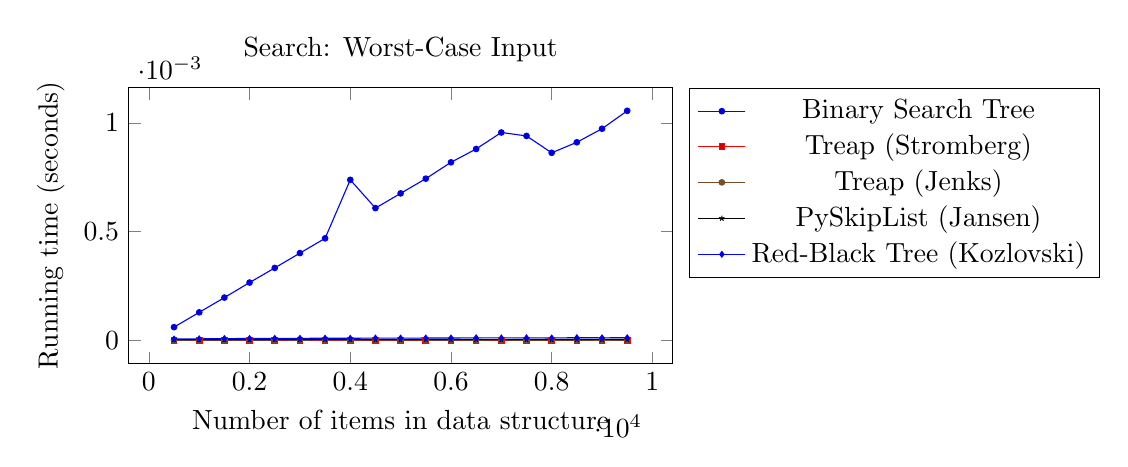
\begin{tikzpicture}
        \begin{axis}[
            xlabel={Number of items in data structure},
            ylabel={Running time (seconds)},
            title={Search: Worst-Case Input},
            width=0.7\textwidth,
            height=2in,
            legend pos=outer north east
        ]
		\addplot coordinates {
			(500, 6.181924962164849e-05)
			(1000, 0.00012983668767364633)
			(1500, 0.00019761017370287543)
			(2000, 0.00026660040809258157)
			(2500, 0.0003338679195560673)
			(3000, 0.00040190945163500635)
			(3500, 0.00046979136078546536)
			(4000, 0.0007382590559659064)
			(4500, 0.0006085247679067552)
			(5000, 0.000676150678020977)
			(5500, 0.0007437856233952989)
			(6000, 0.0008188204467936133)
			(6500, 0.0008801517923697232)
			(7000, 0.0009557708959213329)
			(7500, 0.0009399772612620705)
			(8000, 0.0008625029176360765)
			(8500, 0.000910904806005437)
			(9000, 0.0009731035365513918)
			(9500, 0.0010552701919239826)
		};
		\addplot coordinates {
			(500, 1.075195952200403e-06)
			(1000, 1.0842312123138243e-06)
			(1500, 1.2107248537418513e-06)
			(2000, 1.572135257834617e-06)
			(2500, 1.6594761055088724e-06)
			(3000, 1.3552890153789577e-06)
			(3500, 1.4275710961975108e-06)
			(4000, 1.4275710961975108e-06)
			(4500, 1.5480412309010206e-06)
			(5000, 1.7227229262317679e-06)
			(5500, 1.9245104018494884e-06)
			(6000, 1.716699419489487e-06)
			(6500, 1.2559011542556674e-06)
			(7000, 1.313124468236282e-06)
			(7500, 1.5932175314148367e-06)
			(8000, 1.358300768750098e-06)
			(8500, 1.3733595355880369e-06)
			(9000, 1.578158764576898e-06)
			(9500, 1.551052984272161e-06)
		};
		\addplot coordinates {
			(500, 1.6173115583484333e-06)
			(1000, 1.7468169531653643e-06)
			(1500, 1.8702988412400145e-06)
			(2000, 1.5781587645946615e-06)
			(2500, 2.0479922899241388e-06)
			(3000, 1.870298841222251e-06)
			(3500, 2.0750980702288757e-06)
			(4000, 1.933545661945146e-06)
			(4500, 2.273873792475456e-06)
			(5000, 1.948604428783085e-06)
			(5500, 2.041968783181858e-06)
			(6000, 1.6293585718152315e-06)
			(6500, 1.8401813075463736e-06)
			(7000, 2.1202743707249283e-06)
			(7500, 1.502864930404968e-06)
			(8000, 1.578158764576898e-06)
			(8500, 1.7588639666143991e-06)
			(9000, 1.7227229262140043e-06)
			(9500, 1.7377816930697065e-06)
		};
		\addplot coordinates {
			(500, 5.0025223434424504e-06)
			(1000, 4.300783808801612e-06)
			(1500, 5.035651630489468e-06)
			(2000, 4.2495840015632776e-06)
			(2500, 5.580778990008639e-06)
			(3000, 4.960357796299775e-06)
			(3500, 5.78256646562636e-06)
			(4000, 5.734378411741403e-06)
			(4500, 4.653158952798719e-06)
			(5000, 4.538712324837491e-06)
			(5500, 5.580778990008639e-06)
			(6000, 4.891087468852362e-06)
			(6500, 4.981440069879994e-06)
			(7000, 4.698335253330299e-06)
			(7500, 5.228403846011531e-06)
			(8000, 4.897110975576879e-06)
			(8500, 4.9483107828329765e-06)
			(9000, 5.656072824198332e-06)
			(9500, 5.264544886411926e-06)
		};
		\addplot coordinates {
			(500, 7.2583256157088275e-06)
			(1000, 8.243168966899361e-06)
			(1500, 9.375588233080378e-06)
			(2000, 9.66471655635459e-06)
			(2500, 1.0179726382197884e-05)
			(3000, 1.04447606785385e-05)
			(3500, 1.0986876284686531e-05)
			(4000, 1.070678322152574e-05)
			(4500, 1.1757885146774783e-05)
			(5000, 1.1547062411061404e-05)
			(5500, 1.1857273007915837e-05)
			(6000, 1.1893414048333994e-05)
			(6500, 1.2968610000534397e-05)
			(7000, 1.2366259327034611e-05)
			(7500, 1.2992704027467994e-05)
			(8000, 1.203195470322882e-05)
			(8500, 1.3525784373520367e-05)
			(9000, 1.2851151619202027e-05)
			(9500, 1.3167385722780977e-05)
		};
        \legend{Binary Search Tree, Treap (Stromberg), Treap (Jenks), PySkipList (Jansen), Red-Black Tree (Kozlovski)}
        \end{axis}
    \end{tikzpicture}
    \caption{Average of 100 operations, benchmarked every 500, starting at 500.}
\end{figure}
        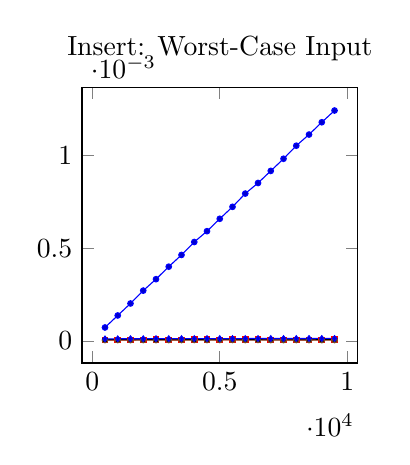
\begin{tikzpicture}
        \begin{axis}[
            title={Insert: Worst-Case Input},
            width=2in,
            height=2in,
        ]
		\addplot coordinates {
			(500, 7.212245789192323e-05)
			(1000, 0.00013702875471527625)
			(1500, 0.000201763381596681)
			(2000, 0.00027111201463712154)
			(2500, 0.0003329101819851965)
			(3000, 0.0004002047992289903)
			(3500, 0.00046372870125665377)
			(4000, 0.000533420674180991)
			(4500, 0.0005918276072372453)
			(5000, 0.0006587035907629501)
			(5500, 0.0007231912538682206)
			(6000, 0.0007947535256337846)
			(6500, 0.0008518051696746554)
			(7000, 0.0009171090179425212)
			(7500, 0.0009825514068652907)
			(8000, 0.001053056553198859)
			(8500, 0.001113264514768879)
			(9000, 0.0011795562181412932)
			(9500, 0.0012428813444467046)
		};
		\addplot coordinates {
			(500, 4.851934675080827e-06)
			(1000, 4.830852401482844e-06)
			(1500, 4.433300956989683e-06)
			(2000, 5.475367622160832e-06)
			(2500, 5.764495945399517e-06)
			(3000, 4.767605580795475e-06)
			(3500, 4.897110975576879e-06)
			(4000, 5.83075451952908e-06)
			(4500, 5.716307891532324e-06)
			(5000, 4.4875125175991574e-06)
			(5500, 6.101812322611977e-06)
			(6000, 5.797625232482062e-06)
			(6500, 5.866895559911711e-06)
			(7000, 5.216356832562497e-06)
			(7500, 5.0416751372495125e-06)
			(8000, 4.285725041981437e-06)
			(8500, 4.586900378740211e-06)
			(9000, 5.565720223188464e-06)
			(9500, 6.011459721548817e-06)
		};
		\addplot coordinates {
			(500, 4.231513481336435e-06)
			(1000, 4.604970898931526e-06)
			(1500, 4.189348934211523e-06)
			(2000, 4.354995369446613e-06)
			(2500, 4.629064925865123e-06)
			(3000, 4.490524270970297e-06)
			(3500, 4.586900378740211e-06)
			(4000, 4.836875908260652e-06)
			(4500, 4.731464540377317e-06)
			(5000, 4.90012272894802e-06)
			(5500, 5.104921957936881e-06)
			(6000, 4.4031834233138055e-06)
			(6500, 5.041675137213985e-06)
			(7000, 4.553771091693193e-06)
			(7500, 4.2797015352391556e-06)
			(8000, 4.61099440563828e-06)
			(8500, 4.592923885482492e-06)
			(9000, 4.351983616039945e-06)
			(9500, 4.270666275125734e-06)
		};
		\addplot coordinates {
			(500, 7.938981876804974e-06)
			(1000, 8.201004419738923e-06)
			(1500, 9.083448156417263e-06)
			(2000, 8.899731200990858e-06)
			(2500, 7.932958370062693e-06)
			(3000, 9.354505959535686e-06)
			(3500, 8.794319833143049e-06)
			(4000, 8.6708379450684e-06)
			(4500, 8.80034333988533e-06)
			(5000, 1.0029138713818498e-05)
			(5500, 9.60146973564946e-06)
			(6000, 9.294270892148404e-06)
			(6500, 8.30641578758673e-06)
			(7000, 1.0315255283757097e-05)
			(7500, 1.0294173010194641e-05)
			(8000, 9.718928116981829e-06)
			(8500, 9.459917327383493e-06)
			(9000, 8.490132743013135e-06)
			(9500, 9.047307116034632e-06)
		};
		\addplot coordinates {
			(500, 1.0550172046421835e-05)
			(1000, 1.1086264145809821e-05)
			(1500, 1.1438639289806928e-05)
			(2000, 1.1637415012089036e-05)
			(2500, 1.1851249501155791e-05)
			(3000, 1.1941602102218952e-05)
			(3500, 1.2122307304274216e-05)
			(4000, 1.213134256435211e-05)
			(4500, 1.2333130040005359e-05)
			(5000, 1.2293977246216059e-05)
			(5500, 1.2402400367435007e-05)
			(6000, 1.240842387414176e-05)
			(6500, 1.2682493430595799e-05)
			(7000, 1.2625270116650712e-05)
			(7500, 1.2673458170517903e-05)
			(8000, 1.264936414354878e-05)
			(8500, 1.3019809807808257e-05)
			(9000, 1.2998727534210275e-05)
			(9500, 1.3022821561143872e-05)
		};
        \end{axis}
    \end{tikzpicture}
    \begin{figure}[h]
    \centering
    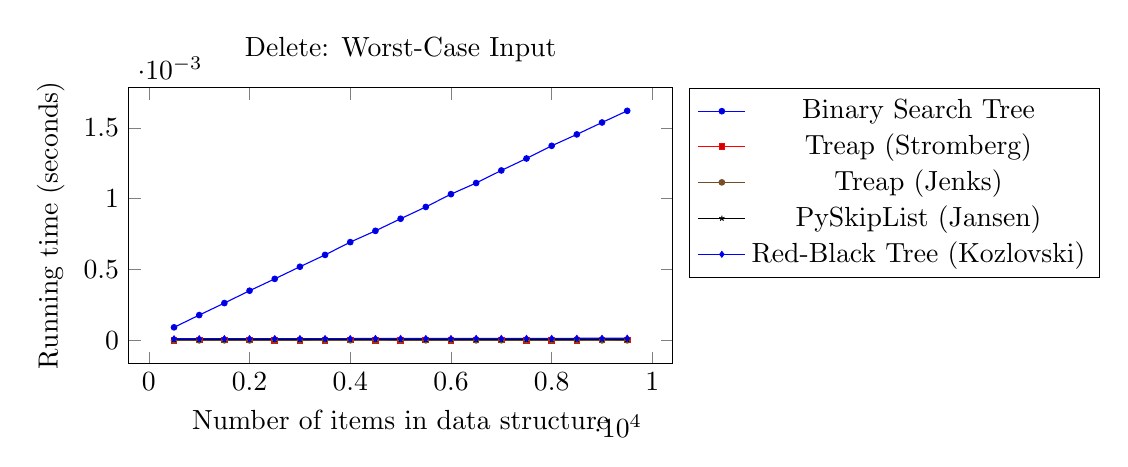
\begin{tikzpicture}
        \begin{axis}[
            xlabel={Number of items in data structure},
            ylabel={Running time (seconds)},
            title={Delete: Worst-Case Input},
            width=0.7\textwidth,
            height=2in,
            legend pos=outer north east
        ]
		\addplot coordinates {
			(9500, 0.0016196366319561762)
			(9000, 0.0015374488943100317)
			(8500, 0.0014535384337376555)
			(8000, 0.001373019207457098)
			(7500, 0.0012837146966034752)
			(7000, 0.0011992832026985311)
			(6500, 0.0011108611355816222)
			(6000, 0.0010323447252904216)
			(5500, 0.0009421125943996245)
			(5000, 0.0008589972367163056)
			(4500, 0.0007737435341419996)
			(4000, 0.0006942031277058547)
			(3500, 0.0006041757960440819)
			(3000, 0.0005206899926965036)
			(2500, 0.00043513210303210316)
			(2000, 0.0003517426757922948)
			(1500, 0.0002646548154171313)
			(1000, 0.00017986793461481908)
			(500, 9.353602433492369e-05)
		};
		\addplot coordinates {
			(9500, 3.0810236949463387e-06)
			(9000, 3.1804115560873923e-06)
			(8500, 2.906341999633355e-06)
			(8000, 2.782860111594232e-06)
			(7500, 2.267850285733175e-06)
			(7000, 3.2496818835170416e-06)
			(6500, 3.475563386103886e-06)
			(6000, 3.035847394414759e-06)
			(5500, 3.5297749467133597e-06)
			(5000, 3.0539179146416017e-06)
			(4500, 2.8430951788749325e-06)
			(4000, 3.168364542673885e-06)
			(3500, 2.8340599187970383e-06)
			(3000, 2.5961314027966864e-06)
			(2500, 1.9516161821542253e-06)
			(2000, 3.882150090745995e-06)
			(1500, 4.228501727965295e-06)
			(1000, 3.430387085572306e-06)
			(500, 2.547943348858439e-06)
		};
		\addplot coordinates {
			(9500, 2.0058277427636993e-06)
			(9000, 1.8100637738882598e-06)
			(8500, 2.1624389178498403e-06)
			(8000, 1.9305339085207154e-06)
			(7500, 2.186532944818964e-06)
			(7000, 2.538908088851599e-06)
			(6500, 2.047992289959666e-06)
			(6000, 2.28290905255335e-06)
			(5500, 2.1323213842094903e-06)
			(5000, 1.975710209052295e-06)
			(4500, 2.1293096308028226e-06)
			(4000, 2.2256857385372085e-06)
			(3500, 1.8401813075996642e-06)
			(3000, 1.8522283210131717e-06)
			(2500, 2.029921769732823e-06)
			(2000, 1.6052645449349256e-06)
			(1500, 1.8733105946466821e-06)
			(1000, 1.7528404598721181e-06)
			(500, 1.8221107873017673e-06)
		};
		\addplot coordinates {
			(9500, 7.1890552882081235e-06)
			(9000, 9.375588233098142e-06)
			(8500, 8.194980912961114e-06)
			(8000, 7.586606732772339e-06)
			(7500, 7.429995557686197e-06)
			(7000, 7.797429468539008e-06)
			(6500, 7.460113091326548e-06)
			(6000, 7.4360190644284786e-06)
			(5500, 6.984256059254789e-06)
			(5000, 7.354701723514267e-06)
			(4500, 9.14669497710463e-06)
			(4000, 9.360529466277967e-06)
			(3500, 9.547258175075513e-06)
			(3000, 7.2733843825290026e-06)
			(2500, 7.652865306866374e-06)
			(2000, 8.032346231132693e-06)
			(1500, 6.987267812590403e-06)
			(1000, 6.86378592455128e-06)
			(500, 6.586704614761629e-06)
		};
		\addplot coordinates {
			(9500, 1.7091700360651885e-05)
			(9000, 1.6308644485150127e-05)
			(8500, 1.637189130576644e-05)
			(8000, 1.5649070497616434e-05)
			(7500, 1.5736411345272927e-05)
			(7000, 1.567617627792117e-05)
			(6500, 1.5757493618835384e-05)
			(6000, 1.50105787836452e-05)
			(5500, 1.5082860864481517e-05)
			(5000, 1.4947331962957832e-05)
			(4500, 1.5022625797129763e-05)
			(4000, 1.4516651231417655e-05)
			(3500, 1.4459427917401513e-05)
			(3000, 1.4450392657394672e-05)
			(2500, 1.4417263370276601e-05)
			(2000, 1.4125123293666774e-05)
			(1500, 1.379383042326765e-05)
			(1000, 1.3634207494703787e-05)
			(500, 1.30830566284601e-05)
		};
        \legend{Binary Search Tree, Treap (Stromberg), Treap (Jenks), PySkipList (Jansen), Red-Black Tree (Kozlovski)}
        \end{axis}
    \end{tikzpicture}
    \caption{Average of 100 operations, benchmarked every 500, starting at 500.}
\end{figure}
    \caption{Average of 100 operations, benchmarked every 500, starting at 500.}
\end{figure}

The more interesting graphs appear when the binary search tree is removed from the data set, as appears below. Here, same worst-case inputs for binary search trees create minor challenges for the various data structures, as they cope in their own ways with the ordered input data. By removing the binary search tree, the benchmarks can once again run at their full scales without issue, which already demonstrates their power to cope with difficult input sets.

\begin{figure}[h]
    \centering
    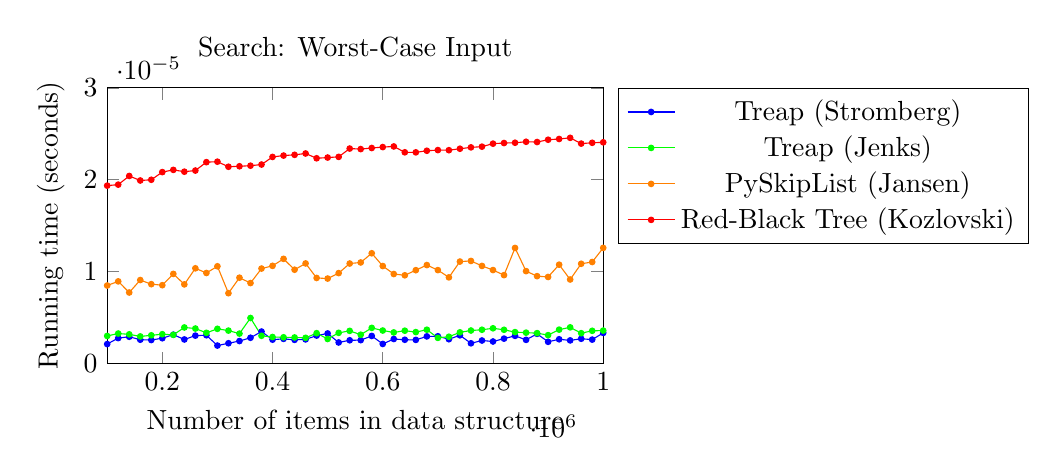
\begin{tikzpicture}
        \begin{axis}[
            title={Search: Worst-Case Input},
            xmin=100000, xmax=1000000,
            ymin=0, ymax=0.00003,
            xlabel={Number of items in data structure},
            ylabel={Running time (seconds)},
            width=0.65\textwidth,
            height=2in,
            legend pos=outer north east,
        ]
		% Stromberg treap
		\addplot[
		    color=blue,
		    mark=*,
	    ]
		coordinates {
			(100000, 2.0991920971591636e-06)
			(120000, 2.7500319998795265e-06)
			(140000, 2.895800862867337e-06)
			(160000, 2.5744467785533407e-06)
			(180000, 2.539811614826859e-06)
			(200000, 2.7355755837153995e-06)
			(220000, 3.121381190094308e-06)
			(240000, 2.6003478575140628e-06)
			(260000, 3.018379224925205e-06)
			(280000, 3.0599414213972054e-06)
			(300000, 1.9359550646398383e-06)
			(320000, 2.1883399968376517e-06)
			(340000, 2.429581441576012e-06)
			(360000, 2.7870765663000617e-06)
			(380000, 3.462311671297513e-06)
			(400000, 2.580169109951402e-06)
			(420000, 2.6675099576092266e-06)
			(440000, 2.5590868363791763e-06)
			(460000, 2.609081942279712e-06)
			(480000, 3.0225956796399166e-06)
			(500000, 3.2548018642755137e-06)
			(520000, 2.273271441801228e-06)
			(540000, 2.5130070098562383e-06)
			(560000, 2.528065776693289e-06)
			(580000, 2.985852288555968e-06)
			(600000, 2.112142636638836e-06)
			(620000, 2.651848840098836e-06)
			(640000, 2.5684232718186096e-06)
			(660000, 2.5557739076740303e-06)
			(680000, 2.9358571826554324e-06)
			(700000, 2.9491088974724634e-06)
			(720000, 2.628357163832362e-06)
			(740000, 3.052110862641122e-06)
			(760000, 2.183220016113374e-06)
			(780000, 2.4877082815688565e-06)
			(800000, 2.3792851603383623e-06)
			(820000, 2.6919051598870423e-06)
			(840000, 2.9945863733225054e-06)
			(860000, 2.5593880117158464e-06)
			(880000, 3.2114326157834937e-06)
			(900000, 2.3452523472862195e-06)
			(920000, 2.619924254403827e-06)
			(940000, 2.4988517690278654e-06)
			(960000, 2.6789546204071258e-06)
			(980000, 2.585289090676568e-06)
			(1000000, 3.3141334056150384e-06)
		};
		% Jenks treap
		\addplot[
		    color=green,
		    mark=*,
	    ]
		coordinates {
			(100000, 2.9831417105263825e-06)
			(120000, 3.246971305518542e-06)
			(140000, 3.1593292825249365e-06)
			(160000, 2.931038377267825e-06)
			(180000, 3.053616739325804e-06)
			(200000, 3.1719786466695153e-06)
			(220000, 3.1027083192149975e-06)
			(240000, 3.908653520362293e-06)
			(260000, 3.7908939636928096e-06)
			(280000, 3.321963964371122e-06)
			(300000, 3.7589693779978007e-06)
			(320000, 3.5668195131499657e-06)
			(340000, 3.2391407467642353e-06)
			(360000, 4.938974347393099e-06)
			(380000, 3.0012122307283563e-06)
			(400000, 2.869297433235829e-06)
			(420000, 2.836168146188811e-06)
			(440000, 2.819302327331741e-06)
			(460000, 2.7777401308597403e-06)
			(480000, 3.2840158719409375e-06)
			(500000, 2.6551617688035376e-06)
			(520000, 3.3228674903789113e-06)
			(540000, 3.5370031548112026e-06)
			(560000, 3.11806826139005e-06)
			(580000, 3.862272518503574e-06)
			(600000, 3.574348896567159e-06)
			(620000, 3.36653791421071e-06)
			(640000, 3.555374850353843e-06)
			(660000, 3.403582480633105e-06)
			(680000, 3.6616897442272036e-06)
			(700000, 2.7750295528292666e-06)
			(720000, 2.898511440900364e-06)
			(740000, 3.3770790509990434e-06)
			(760000, 3.574951247241387e-06)
			(780000, 3.658677990859616e-06)
			(800000, 3.817999744001099e-06)
			(820000, 3.6529556594615544e-06)
			(840000, 3.4005707272619643e-06)
			(860000, 3.34184153659578e-06)
			(880000, 3.290340554013227e-06)
			(900000, 3.074397837561804e-06)
			(920000, 3.672833231686212e-06)
			(940000, 3.919797007821302e-06)
			(960000, 3.285220573285841e-06)
			(980000, 3.5430266615499305e-06)
			(1000000, 3.56862656517265e-06)
		};
		% PySkipList
		\addplot[
		    color=orange,
		    mark=*,
	    ]
        coordinates {
			(100000, 8.475375151530073e-06)
			(120000, 8.927740507328253e-06)
			(140000, 7.714305075555927e-06)
			(160000, 9.072605844309578e-06)
			(180000, 8.622649891201206e-06)
			(200000, 8.511817367274687e-06)
			(220000, 9.742720968581864e-06)
			(240000, 8.598857039597619e-06)
			(260000, 1.0351095148820376e-05)
			(280000, 9.841205303700917e-06)
			(300000, 1.057035079397295e-05)
			(320000, 7.638408890695557e-06)
			(340000, 9.329809581892334e-06)
			(360000, 8.743120025901164e-06)
			(380000, 1.0323085842500745e-05)
			(400000, 1.0617936497183678e-05)
			(420000, 1.137900657315072e-05)
			(440000, 1.0196291025728498e-05)
			(460000, 1.0880862566168047e-05)
			(480000, 9.299993223557124e-06)
			(500000, 9.23403582481086e-06)
			(520000, 9.826748887533655e-06)
			(540000, 1.0870923780053943e-05)
			(560000, 1.09859727586894e-05)
			(580000, 1.1988886630078354e-05)
			(600000, 1.0599263626303922e-05)
			(620000, 9.728565727755266e-06)
			(640000, 9.589723897505564e-06)
			(660000, 1.0147500621172866e-05)
			(680000, 1.0703169117476819e-05)
			(700000, 1.015322295257448e-05)
			(720000, 9.363240044272913e-06)
			(740000, 1.1084155918467786e-05)
			(760000, 1.1151016843228945e-05)
			(780000, 1.0610708289092941e-05)
			(800000, 1.0159246459309657e-05)
			(820000, 9.608396768385318e-06)
			(840000, 1.2567444451974553e-05)
			(860000, 1.0043293954659305e-05)
			(880000, 9.495757192439669e-06)
			(900000, 9.407813994116055e-06)
			(920000, 1.0746237190637941e-05)
			(940000, 9.131937385646438e-06)
			(960000, 1.08438179997421e-05)
			(980000, 1.1035967864593487e-05)
			(1000000, 1.2574070309383956e-05)
		};
		% Red-black tree
		\addplot[
		    color=red, 
		    mark=*,
	    ]
	    coordinates {
			(100000, 1.9352021262982078e-05)
			(120000, 1.9463154962238604e-05)
			(140000, 2.0406134941616472e-05)
			(160000, 1.9913110915346976e-05)
			(180000, 1.9992922379586275e-05)
			(200000, 2.0828081588398107e-05)
			(220000, 2.106902185779802e-05)
			(240000, 2.087235436290058e-05)
			(260000, 2.099613742630879e-05)
			(280000, 2.1910806924019254e-05)
			(300000, 2.19620067312718e-05)
			(320000, 2.1411157040354566e-05)
			(340000, 2.146175449692578e-05)
			(360000, 2.1525904843649357e-05)
			(380000, 2.1650290257731798e-05)
			(400000, 2.247942595980845e-05)
			(420000, 2.26270018748167e-05)
			(440000, 2.2708319215738014e-05)
			(460000, 2.285378690339712e-05)
			(480000, 2.23318500447931e-05)
			(500000, 2.241286621038796e-05)
			(520000, 2.248575064187719e-05)
			(540000, 2.33925895808369e-05)
			(560000, 2.3333559214833597e-05)
			(580000, 2.3451318771506634e-05)
			(600000, 2.355100780798125e-05)
			(620000, 2.3621181661425794e-05)
			(640000, 2.2983292298192737e-05)
			(660000, 2.2979075843480247e-05)
			(680000, 2.3152251662111212e-05)
			(700000, 2.3224533742933318e-05)
			(720000, 2.3214293781478547e-05)
			(740000, 2.3372712008622897e-05)
			(760000, 2.3520589098950494e-05)
			(780000, 2.359829233583355e-05)
			(800000, 2.3925368751548602e-05)
			(820000, 2.3992530851643324e-05)
			(840000, 2.4024756612675445e-05)
			(860000, 2.413016798054457e-05)
			(880000, 2.4101556323557817e-05)
			(900000, 2.4352736554405395e-05)
			(920000, 2.4435258596682275e-05)
			(940000, 2.4558138134068485e-05)
			(960000, 2.393259695963934e-05)
			(980000, 2.4019335456614497e-05)
			(1000000, 2.4072041140556168e-05)
		};
        \legend{Treap (Stromberg), Treap (Jenks), PySkipList (Jansen), Red-Black Tree (Kozlovski)}
        \end{axis}
    \end{tikzpicture}
    \caption{Average of 1000 operations, benchmarked every 20000, starting at 100000.}
\end{figure}

The first graph, search, presents a great deal more noise than the randomized input search benchmarks. This, I attribute simply to the challenges and inefficiencies inherent in coping with sorted inputs to these data structures. The specifics are surprising and don't seem to have simple explanations. The two treaps perform almost identically, in contrast with the marked performance difference on search with randomized inputs. This suggests that ordered inputs to insert may cause the trees to develop more similar geometries than random inputs. PySkipList is by far the noisiest on search, which suggests a high degree of unpredictability in its performance, even as it maintains logarithmic complexity overall. Lastly, the red-black tree is consistent but slower than the rest. 

The relative speeds of the three data structures remain unchanged: the treaps are fastest, the skiplist is significantly slower, and the red-black tree is slower still. While these are not provable general statements about the three data structures, they do provide insight into the impact of ordered inputs (to both insert and search) on the performance of searches, which is to say that the data structures are only very modestly affected. Finally, it is worth noting that, compared to search with randomized inputs, the red-black tree and Stromberg treap are both noticeably slower, whereas the Jenks treap and PySkipList remain about the same in their overall speeds.

\begin{figure}[h]
    \centering
    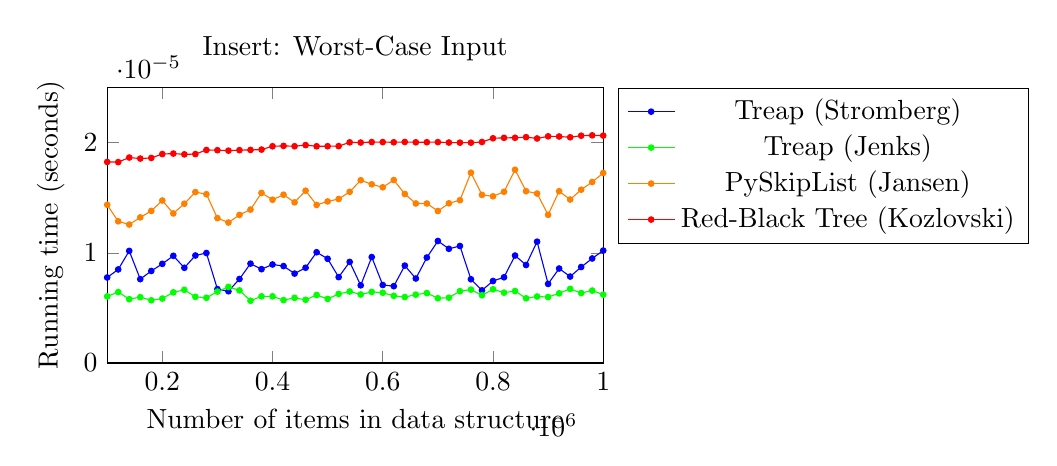
\begin{tikzpicture}
        \begin{axis}[
            title={Insert: Worst-Case Input},
            xmin=100000, xmax=1000000,
            ymin=0, ymax=0.000025,
            xlabel={Number of items in data structure},
            ylabel={Running time (seconds)},
            width=0.65\textwidth,
            height=2in,
            legend pos=outer north east,
        ]
		% Stromberg treap
		\addplot[
		    color=blue,
		    mark=*,
	    ]
		coordinates {
			(100000, 7.761288428090623e-06)
			(120000, 8.494349197744194e-06)
			(140000, 1.0177015804175793e-05)
			(160000, 7.613712513082294e-06)
			(180000, 8.354905016828118e-06)
			(200000, 9.000624938823698e-06)
			(220000, 9.730673955109736e-06)
			(240000, 8.643732164772988e-06)
			(260000, 9.759285612101153e-06)
			(280000, 9.985468290001798e-06)
			(300000, 6.709885327490727e-06)
			(320000, 6.514121358601965e-06)
			(340000, 7.626964227899435e-06)
			(360000, 9.022008387733038e-06)
			(380000, 8.518744400020761e-06)
			(400000, 8.944305150850873e-06)
			(420000, 8.799439813873545e-06)
			(440000, 8.116374150120897e-06)
			(460000, 8.649755671508164e-06)
			(480000, 1.0054437442117869e-05)
			(500000, 9.462627905400645e-06)
			(520000, 7.797730643837042e-06)
			(540000, 9.179221913517388e-06)
			(560000, 7.0508158086939335e-06)
			(580000, 9.618034379164974e-06)
			(600000, 7.081535693042262e-06)
			(620000, 6.974919623831788e-06)
			(640000, 8.842507887028894e-06)
			(660000, 7.67123700240191e-06)
			(680000, 9.577074533366314e-06)
			(700000, 1.1075120658369463e-05)
			(720000, 1.0367057441666106e-05)
			(740000, 1.062275530256862e-05)
			(760000, 7.605279603652982e-06)
			(780000, 6.59905280356643e-06)
			(800000, 7.4444519738277034e-06)
			(820000, 7.785081279694239e-06)
			(840000, 9.755069157386664e-06)
			(860000, 8.897622973654152e-06)
			(880000, 1.1016993818374843e-05)
			(900000, 7.181525904842445e-06)
			(920000, 8.577172415350276e-06)
			(940000, 7.847424574400463e-06)
			(960000, 8.713906018234852e-06)
			(980000, 9.49003486104516e-06)
			(1000000, 1.020803686385996e-05)
		};
		% Jenks treap
		\addplot[
		    color=green,
		    mark=*,
	    ]
		coordinates {
			(100000, 6.048203112648309e-06)
			(120000, 6.441538102443189e-06)
			(140000, 5.797324057132514e-06)
			(160000, 5.981041012551813e-06)
			(180000, 5.6937197412896266e-06)
			(200000, 5.852439143758659e-06)
			(220000, 6.4165405494946985e-06)
			(240000, 6.643927928742244e-06)
			(260000, 6.006640916176309e-06)
			(280000, 5.924118873902984e-06)
			(300000, 6.4821967729074e-06)
			(320000, 6.910769277105544e-06)
			(340000, 6.59423399817527e-06)
			(360000, 5.653663421504973e-06)
			(380000, 6.056033671402617e-06)
			(400000, 6.054527794720599e-06)
			(420000, 5.7108867354855876e-06)
			(440000, 5.915384789140887e-06)
			(460000, 5.737691340456763e-06)
			(480000, 6.176804981439687e-06)
			(500000, 5.819309856718746e-06)
			(520000, 6.272578738528267e-06)
			(540000, 6.491834383684392e-06)
			(560000, 6.22168010661639e-06)
			(580000, 6.456596869281128e-06)
			(600000, 6.38220656110633e-06)
			(620000, 6.101812322590661e-06)
			(640000, 5.989775097315686e-06)
			(660000, 6.208428391797582e-06)
			(680000, 6.35028197541132e-06)
			(700000, 5.8822555020974225e-06)
			(720000, 5.928937679293256e-06)
			(740000, 6.522855443368059e-06)
			(760000, 6.66440785164113e-06)
			(780000, 6.1518074284911965e-06)
			(800000, 6.692417157957209e-06)
			(820000, 6.387928892504391e-06)
			(840000, 6.535504807512638e-06)
			(860000, 5.875328469350905e-06)
			(880000, 6.0385655018713184e-06)
			(900000, 5.988570395970783e-06)
			(920000, 6.32799500048975e-06)
			(940000, 6.731268776398735e-06)
			(960000, 6.353293728775355e-06)
			(980000, 6.575259951961954e-06)
			(1000000, 6.2042119370850915e-06)
		};
		% PySkipList
		\addplot[
		    color=orange,
		    mark=*,
	    ]
        coordinates {
			(100000, 1.4357931828961057e-05)
			(120000, 1.2862295106653932e-05)
			(140000, 1.2569853854667912e-05)
			(160000, 1.3219187880704197e-05)
			(180000, 1.380587743669537e-05)
			(200000, 1.4750062117414586e-05)
			(220000, 1.3576381830091577e-05)
			(240000, 1.4458825566777022e-05)
			(260000, 1.551504747276056e-05)
			(280000, 1.5323198783249835e-05)
			(300000, 1.3154134007965723e-05)
			(320000, 1.2751462582730966e-05)
			(340000, 1.3443262331247042e-05)
			(360000, 1.392574522072465e-05)
			(380000, 1.5440054813915083e-05)
			(400000, 1.4819031269524886e-05)
			(420000, 1.5275311904701992e-05)
			(440000, 1.4582608630178129e-05)
			(460000, 1.5640035237517225e-05)
			(480000, 1.4347390692172724e-05)
			(500000, 1.4667540075144813e-05)
			(520000, 1.48870968956345e-05)
			(540000, 1.553853914902703e-05)
			(560000, 1.6591146950972303e-05)
			(580000, 1.6219496585421213e-05)
			(600000, 1.5949342308353208e-05)
			(620000, 1.6608615120510704e-05)
			(640000, 1.5341871654136694e-05)
			(660000, 1.4479907840346584e-05)
			(680000, 1.4477498437656777e-05)
			(700000, 1.3795035124573474e-05)
			(720000, 1.4496773659203655e-05)
			(740000, 1.4777167897719324e-05)
			(760000, 1.7273309088722043e-05)
			(780000, 1.5260554313208276e-05)
			(800000, 1.5129844217057098e-05)
			(820000, 1.554275560373952e-05)
			(840000, 1.7545872768479855e-05)
			(860000, 1.55969671643561e-05)
			(880000, 1.5382530324593802e-05)
			(900000, 1.3448984662645102e-05)
			(920000, 1.559395541098496e-05)
			(940000, 1.4838908841753096e-05)
			(960000, 1.573068901387842e-05)
			(980000, 1.6430319321152355e-05)
			(1000000, 1.724770918509222e-05)
		};
		% Red-black tree
		\addplot[
		    color=red, 
		    mark=*,
	    ]
	    coordinates {
			(100000, 1.825032188114051e-05)
			(120000, 1.8234961938965455e-05)
			(140000, 1.864968037767767e-05)
			(160000, 1.8556918373953124e-05)
			(180000, 1.8614442863274405e-05)
			(200000, 1.8966215656597283e-05)
			(220000, 1.9010187255766197e-05)
			(240000, 1.8937905174944092e-05)
			(260000, 1.8962601552559022e-05)
			(280000, 1.933545661945857e-05)
			(300000, 1.931738609925304e-05)
			(320000, 1.9275823902781043e-05)
			(340000, 1.932130137863197e-05)
			(360000, 1.9341480126193743e-05)
			(380000, 1.9370995309195392e-05)
			(400000, 1.9673977697969747e-05)
			(420000, 1.970529993299408e-05)
			(440000, 1.967548357464466e-05)
			(460000, 1.978029259183245e-05)
			(480000, 1.9672772996614184e-05)
			(500000, 1.9678194152689345e-05)
			(520000, 1.9688434114129906e-05)
			(540000, 2.0028762244663766e-05)
			(560000, 2.0009185847769118e-05)
			(580000, 2.0054362148286485e-05)
			(600000, 2.0052253920923134e-05)
			(620000, 2.003538810205896e-05)
			(640000, 2.006279505771147e-05)
			(660000, 2.0034183400724713e-05)
			(680000, 2.0041411608801242e-05)
			(700000, 2.0049543342892662e-05)
			(720000, 2.001008937378401e-05)
			(740000, 2.0000752938344134e-05)
			(760000, 1.99977411849801e-05)
			(780000, 2.006068683036233e-05)
			(800000, 2.039890673353284e-05)
			(820000, 2.043836070264149e-05)
			(840000, 2.0443179508035315e-05)
			(860000, 2.0500402822008822e-05)
			(880000, 2.0382040914668665e-05)
			(900000, 2.0575395480861403e-05)
			(920000, 2.0560336714027018e-05)
			(940000, 2.0489560509886927e-05)
			(960000, 2.0632618794849123e-05)
			(980000, 2.0663338679199227e-05)
			(1000000, 2.063984700293986e-05)
		};
        \legend{Treap (Stromberg), Treap (Jenks), PySkipList (Jansen), Red-Black Tree (Kozlovski)}
        \end{axis}
    \end{tikzpicture}
    \caption{Average of 1000 operations, benchmarked every 20000, starting at 100000.}
\end{figure}

Insert on ordered data presents a more interesting picture still. First, the red-black tree, whose performance on random data sat squarely between the two treaps, is now in last place by a wide margin. This makes sense: sorted input is a worst-case scenario for red-black trees, too, because they will need to rotate almost constantly to maintain balance. Yet, it remains clearly and visibly $O(\log n)$ even in this case---an impressive feat. Being deterministic, it exhibits very smooth worst-case performance, but it is indeed far slower than its randomized counterparts.

The remaining three data structures are plagued by differing levels of noise, but their relative performance is essentially unchanged compared to the randomized input insert benchmark. The most noteworthy aspect of their performance is perhaps the consistency of Jenks relative to Stromberg. While Stromberg straddles the line its randomized benchmark cut, with wide and erratic variations in running time, Jenks is quite consistent.

\begin{figure}[h]
    \centering
    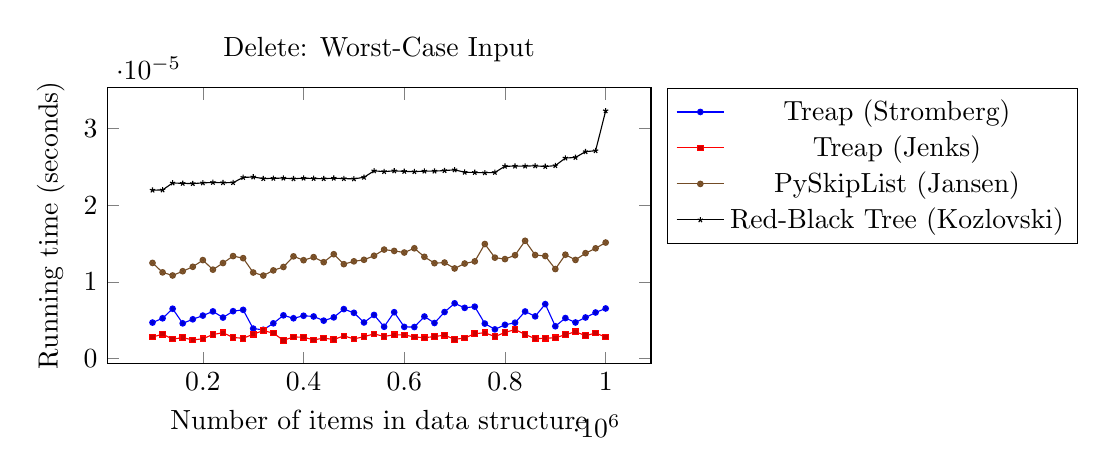
\begin{tikzpicture}
        \begin{axis}[
            xlabel={Number of items in data structure},
            ylabel={Running time (seconds)},
            title={Delete: Worst-Case Input},
            width=0.7\textwidth,
            height=2in,
            legend pos=outer north east
        ]
		\addplot coordinates {
			(1000000, 6.540323612899357e-06)
			(980000, 6.015375000940182e-06)
			(960000, 5.3666433255781245e-06)
			(940000, 4.715201072183817e-06)
			(920000, 5.290747140717756e-06)
			(900000, 4.225188799289015e-06)
			(880000, 7.10954499935923e-06)
			(860000, 5.512412188565463e-06)
			(840000, 6.148494499784718e-06)
			(820000, 4.6823729604792415e-06)
			(800000, 4.410110456054994e-06)
			(780000, 3.814987990633512e-06)
			(760000, 4.5706369105431575e-06)
			(740000, 6.7758427262383235e-06)
			(720000, 6.62043625247577e-06)
			(700000, 7.210438737173419e-06)
			(680000, 6.075610068291937e-06)
			(660000, 4.645027218719733e-06)
			(640000, 5.4934381423521475e-06)
			(620000, 4.121283308109014e-06)
			(600000, 4.1396550036516545e-06)
			(580000, 6.0521183920254625e-06)
			(560000, 4.157725523857181e-06)
			(540000, 5.697032669994328e-06)
			(520000, 4.718514000888519e-06)
			(500000, 5.973511629132844e-06)
			(480000, 6.4581027459666985e-06)
			(460000, 5.3795938650580415e-06)
			(440000, 4.951021360861674e-06)
			(420000, 5.499160473748432e-06)
			(400000, 5.59162130213231e-06)
			(380000, 5.2648460617561456e-06)
			(360000, 5.642821109379526e-06)
			(340000, 4.603465022249509e-06)
			(320000, 3.762884657374954e-06)
			(300000, 3.916182903781262e-06)
			(280000, 6.360220761521873e-06)
			(260000, 6.187044942890907e-06)
			(240000, 5.356403364128681e-06)
			(220000, 6.159939162580841e-06)
			(200000, 5.613607101713214e-06)
			(180000, 5.130220686227816e-06)
			(160000, 4.6013567948932635e-06)
			(140000, 6.505688449172098e-06)
			(120000, 5.261231957716106e-06)
			(100000, 4.7022505327039e-06)
		};
		\addplot coordinates {
			(1000000, 2.807556489198504e-06)
			(980000, 3.339733309239534e-06)
			(960000, 2.9942851979818385e-06)
			(940000, 3.5095961991657988e-06)
			(920000, 3.120176488746296e-06)
			(900000, 2.7259379729400733e-06)
			(880000, 2.6548605934664236e-06)
			(860000, 2.606070188910792e-06)
			(840000, 3.154510477138217e-06)
			(820000, 3.794809243068187e-06)
			(800000, 3.414123617417886e-06)
			(780000, 2.873815063285434e-06)
			(760000, 3.3728625962829994e-06)
			(740000, 3.2548018642764022e-06)
			(720000, 2.6822675491118275e-06)
			(700000, 2.5211387439476595e-06)
			(680000, 3.0581343693754093e-06)
			(660000, 2.8861632520893464e-06)
			(640000, 2.723829745580275e-06)
			(620000, 2.8337587434954514e-06)
			(600000, 3.085240149683699e-06)
			(580000, 3.1144541573482343e-06)
			(560000, 2.8921867588280747e-06)
			(540000, 3.22679255795677e-06)
			(520000, 2.8590574717846094e-06)
			(500000, 2.573844427878669e-06)
			(480000, 2.968685294359119e-06)
			(460000, 2.4934306129686946e-06)
			(440000, 2.672027587660608e-06)
			(420000, 2.4458449097615187e-06)
			(400000, 2.796413001739495e-06)
			(380000, 2.8268317107489336e-06)
			(360000, 2.3807910370230445e-06)
			(340000, 3.3340109778414727e-06)
			(320000, 3.6541603608100103e-06)
			(300000, 3.1885432901930246e-06)
			(280000, 2.651246489424608e-06)
			(260000, 2.7629825393589157e-06)
			(240000, 3.374368472965017e-06)
			(220000, 3.1524022497784187e-06)
			(200000, 2.5858914413490198e-06)
			(180000, 2.438917877015001e-06)
			(160000, 2.735274408379951e-06)
			(140000, 2.547340998244607e-06)
			(120000, 3.1882421148523577e-06)
			(100000, 2.815688223289925e-06)
		};
		\addplot coordinates {
			(1000000, 1.5134663022443816e-05)
			(980000, 1.4379315277871285e-05)
			(960000, 1.3750461174737439e-05)
			(940000, 1.286922213940045e-05)
			(920000, 1.3549577225120402e-05)
			(900000, 1.1679880734568825e-05)
			(880000, 1.3381521387209715e-05)
			(860000, 1.3506810327299944e-05)
			(840000, 1.536265275236559e-05)
			(820000, 1.3481210423677225e-05)
			(800000, 1.2975838208610924e-05)
			(780000, 1.316708454744031e-05)
			(760000, 1.4941007280910412e-05)
			(740000, 1.2678276975897517e-05)
			(720000, 1.2399388614070973e-05)
			(700000, 1.1756379270096317e-05)
			(680000, 1.2525279904828324e-05)
			(660000, 1.2444263739247674e-05)
			(640000, 1.3271592389301645e-05)
			(620000, 1.4386844661288478e-05)
			(600000, 1.3832983217007212e-05)
			(580000, 1.4041998900708563e-05)
			(560000, 1.4215777070013757e-05)
			(540000, 1.341073539488491e-05)
			(520000, 1.2884582081575501e-05)
			(500000, 1.2684601657966255e-05)
			(480000, 1.2318974799157445e-05)
			(460000, 1.3612824045836192e-05)
			(440000, 1.257376913404329e-05)
			(420000, 1.32312348941781e-05)
			(400000, 1.2834285800337853e-05)
			(380000, 1.3331225105979172e-05)
			(360000, 1.1949432660955494e-05)
			(340000, 1.150309081189249e-05)
			(320000, 1.0832373336945977e-05)
			(300000, 1.1228117729437769e-05)
			(280000, 1.3099922447352697e-05)
			(260000, 1.3365860269701102e-05)
			(240000, 1.2466851889499253e-05)
			(220000, 1.1602177497685773e-05)
			(200000, 1.2845128112452641e-05)
			(180000, 1.1972623161895512e-05)
			(160000, 1.1396173567348456e-05)
			(140000, 1.0841709772385854e-05)
			(120000, 1.124588707430263e-05)
			(100000, 1.2480705954992288e-05)
		};
		\addplot coordinates {
			(1000000, 3.2303464269304525e-05)
			(980000, 2.710608148298377e-05)
			(960000, 2.6977780789522398e-05)
			(940000, 2.6227553025677252e-05)
			(920000, 2.6147741561445058e-05)
			(900000, 2.5159585281556927e-05)
			(880000, 2.5046945705625488e-05)
			(860000, 2.513217832590442e-05)
			(840000, 2.5103867844265438e-05)
			(820000, 2.5093025532143543e-05)
			(800000, 2.5079773817324737e-05)
			(780000, 2.4275334492855906e-05)
			(760000, 2.4229555841671415e-05)
			(740000, 2.4267503934112257e-05)
			(720000, 2.430183792249352e-05)
			(700000, 2.4609639116647485e-05)
			(680000, 2.4513263008898888e-05)
			(660000, 2.444851031148687e-05)
			(640000, 2.4445197382789276e-05)
			(620000, 2.4374120003315625e-05)
			(600000, 2.441297162175715e-05)
			(580000, 2.4477724319154957e-05)
			(560000, 2.4382854088074168e-05)
			(540000, 2.4476218442472943e-05)
			(520000, 2.3639252181638427e-05)
			(500000, 2.343475412799023e-05)
			(480000, 2.3468786941037934e-05)
			(460000, 2.3522697326313845e-05)
			(440000, 2.346216108362853e-05)
			(420000, 2.3487459811917688e-05)
			(400000, 2.352962435907102e-05)
			(380000, 2.3451619946854407e-05)
			(360000, 2.3532334937101496e-05)
			(340000, 2.3508542085480144e-05)
			(320000, 2.34681845903566e-05)
			(300000, 2.367960967676197e-05)
			(280000, 2.3621181661440004e-05)
			(260000, 2.2939019523690263e-05)
			(240000, 2.2933598367629316e-05)
			(220000, 2.2970944109388824e-05)
			(200000, 2.290860081467372e-05)
			(180000, 2.2820356441016542e-05)
			(160000, 2.2848968098003298e-05)
			(140000, 2.289896320390028e-05)
			(120000, 2.199182308960701e-05)
			(100000, 2.19620067312718e-05)
		};
        \legend{Treap (Stromberg), Treap (Jenks), PySkipList (Jansen), Red-Black Tree (Kozlovski)}
        \end{axis}
    \end{tikzpicture}
    \caption{Average of 1000 operations, benchmarked every 20000, starting at 100000.}
\end{figure}

Delete is much the same story: worst-case but very consistent performance for the red-black tree, while the randomized data structures have some noise but are still relatively consistent. Again, Jenks is much more stable than Stromberg in its running times.

\section{Benchmark: Random Sequence of Operations}

In searching for data structure implementations in Python, I found a plethora of references to the Sorted Containers package and its SortedList class in particular. The advice seemed to be: if you need a sorted data structure, forget trees and use SortedList. It seems fitting, after investigating the performance of these well-known data structures relative to one another, to benchmark them all against the Python-specific data structure commonly used in practice. 

The SortedList class leverages Python's very fast implementation of lists (for sizes up to 10,000) by storing a list of sorted sublists that can each be individually managed very quickly. To locate elements, SortedList performs a binary search on the lists' maxima and the performs a binary search on the appropriate list. It is also designed around the observation that "a lot of time has been spent optimizing mem-copy/mem-move-like operations both in hardware and software."\footnote{\url{http://www.grantjenks.com/docs/sortedcontainers/implementation.html}}

This final benchmark is also structured somewhat differently than the rest in order to provide a different perspective on the data structures examined so far. For this benchmark, each data structure is subjected to the same, randomly generated sequence of search, insert, and delete operations. As before, no duplicates are inserted, no absent elements are searched for, and no absent elements are deleted. This benchmark does not aim to mimic a real-world workflow; it simply aims to put the data structures through their paces in a less static way and observe their performance under varied conditions.

% Custom 2-ordinate graph. See pgfplots manual, section Two Ordinates, for details.
\begin{figure}[h]
    \centering
    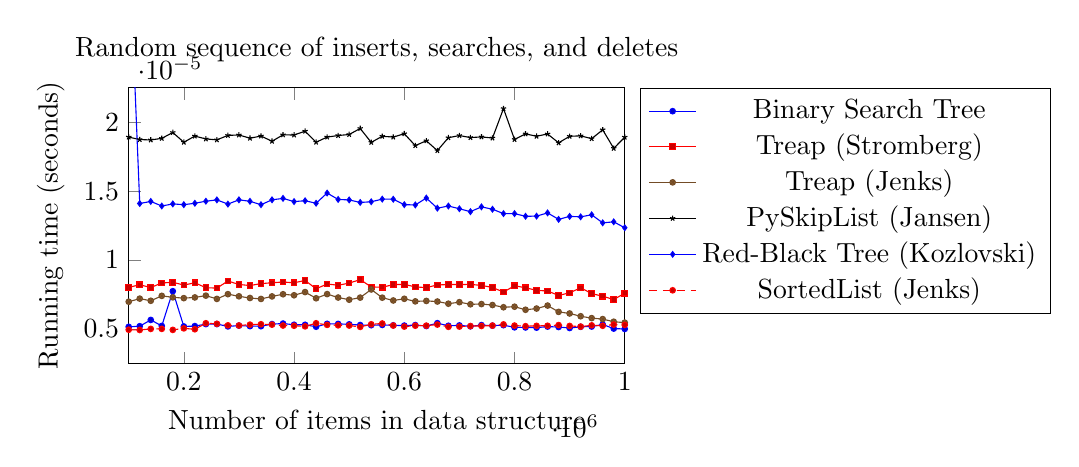
\begin{tikzpicture}
        \pgfplotsset{set layers}
% 	    \begin{axis}[
% 	        scale only axis,
%             xmin=100000, xmax=1000000,
%             ymin=0,
%             width=0.7\textwidth,
%             height=2in,
%             axis y line=right,
%             hide x axis,
%             yticklabels={,,}, % Hide ytick labels
%             scaled ticks=false, % Hide ytick scale label
%             ytick=\empty, % Hide yticks themselves
%             % xtick style={middle left},
%             % Make legend position same as other graph so other % graph's legend will hide this one. Then we'll copy % entries from this graph.
%             legend pos=outer north east
%         ]
%     		\addplot coordinates {
%     			(100000, 10087.0)
%     			(120000, 11822.0)
%     			(140000, 13649.0)
%     			(160000, 15655.0)
%     			(180000, 17653.0)
%     			(200000, 19563.0)
%     			(220000, 21616.0)
%     			(240000, 23682.0)
%     			(260000, 25781.0)
%     			(280000, 27700.5)
%     			(300000, 29626.0)
%     			(320000, 31867.0)
%     			(340000, 33777.5)
%     			(360000, 35913.0)
%     			(380000, 37982.0)
%     			(400000, 40018.5)
%    			(420000, 42128.0)
%    			(440000, 44087.0)
%    			(460000, 46319.0)
%    			(480000, 48257.0)
%    			(500000, 50304.0)
%    			(520000, 52345.0)
%    			(540000, 54439.0)
%    			(560000, 56455.0)
%    			(580000, 58622.0)
%    			(600000, 60617.5)
%    			(620000, 62579.0)
%    			(640000, 64485.0)
%    			(660000, 66354.0)
%    			(680000, 68442.0)
%    			(700000, 70504.0)
%    			(720000, 72499.5)
%    			(740000, 74594.0)
%    			(760000, 76683.0)
%    			(780000, 78700.0)
%    			(800000, 80783.0)
%    			(820000, 82852.0)
%    			(840000, 84952.0)
%    			(860000, 87044.0)
%    			(880000, 89179.5)
%    			(900000, 91006.0)
%    			(920000, 92791.0)
%    			(940000, 94675.0)
%    			(960000, 96586.0)
%    			(980000, 98539.0)
%    			(1000000, 100518.0)
%    		};
%    		\label{data_structure_size}
%    		\addlegendentry{Data Structure Size}
%        \end{axis}
        \begin{axis}[
            xmin=100000, xmax=1000000,
            ymin=0.0000025, ymax=0.0000225,
            xlabel={Number of items in data structure},
            ylabel={Running time (seconds)},
            ytick pos=left,
            title={Random sequence of inserts, searches, and deletes},
            width=0.65\textwidth,
            height=2in,
            legend pos=outer north east,
        ]
    		\addplot coordinates {
    			(100000, 5.151302959802706e-06)
    			(120000, 5.196479260121123e-06)
    			(140000, 5.651856369695452e-06)
    			(160000, 5.2163568325340744e-06)
    			(180000, 7.739001453046513e-06)
    			(200000, 5.178408739993756e-06)
    			(220000, 5.204912170029274e-06)
    			(240000, 5.347066928607092e-06)
    			(260000, 5.350078682113235e-06)
    			(280000, 5.1823240196426925e-06)
    			(300000, 5.239547333530936e-06)
    			(320000, 5.202201592055644e-06)
    			(340000, 5.197081611186149e-06)
    			(360000, 5.348873980437929e-06)
    			(380000, 5.38832794973132e-06)
    			(400000, 5.301890628288674e-06)
    			(420000, 5.2994812253928105e-06)
    			(440000, 5.1594346941783444e-06)
    			(460000, 5.368751552850881e-06)
    			(480000, 5.365438624266972e-06)
    			(500000, 5.331104635843076e-06)
    			(520000, 5.282615406486002e-06)
    			(540000, 5.269966042760643e-06)
    			(560000, 5.288337737965776e-06)
    			(580000, 5.259123730411375e-06)
    			(600000, 5.2413543858165215e-06)
    			(620000, 5.278700127291813e-06)
    			(640000, 5.2100321504440215e-06)
    			(660000, 5.4154337299223695e-06)
    			(680000, 5.22689796935083e-06)
    			(700000, 5.255208450762439e-06)
    			(720000, 5.1880463506677185e-06)
    			(740000, 5.276893075006228e-06)
    			(760000, 5.237740281700099e-06)
    			(780000, 5.27297779581204e-06)
    			(800000, 5.11425839340518e-06)
    			(820000, 5.105223133341496e-06)
    			(840000, 5.0922725936288774e-06)
    			(860000, 5.1669640774889556e-06)
    			(880000, 5.137750069479807e-06)
    			(900000, 5.065166813437827e-06)
    			(920000, 5.15431471330885e-06)
    			(940000, 5.17208405835845e-06)
    			(960000, 5.3208646741040865e-06)
    			(980000, 5.023303441703319e-06)
    			(1000000, 4.996498837044783e-06)
    		};
    		\addplot coordinates {
    			(100000, 8.019696866995218e-06)
    			(120000, 8.201305594866425e-06)
    			(140000, 8.00493927545176e-06)
    			(160000, 8.336232146120892e-06)
    			(180000, 8.383817848880427e-06)
    			(200000, 8.18263272412878e-06)
    			(220000, 8.348881509846252e-06)
    			(240000, 7.99198873619389e-06)
    			(260000, 7.963377079249767e-06)
    			(280000, 8.476881028400384e-06)
    			(300000, 8.22600197261636e-06)
    			(320000, 8.149503436925443e-06)
    			(340000, 8.288345267374098e-06)
    			(360000, 8.35098973766435e-06)
    			(380000, 8.40520129804645e-06)
    			(400000, 8.347375633547926e-06)
    			(420000, 8.519045575212659e-06)
    			(440000, 7.912478447451576e-06)
    			(460000, 8.259131259819696e-06)
    			(480000, 8.171489236701746e-06)
    			(500000, 8.322980431330507e-06)
    			(520000, 8.582593571190955e-06)
    			(540000, 8.048007348406827e-06)
    			(560000, 8.024515672786947e-06)
    			(580000, 8.215762011332118e-06)
    			(600000, 8.234434882069764e-06)
    			(620000, 8.047404997796548e-06)
    			(640000, 8.00012047011478e-06)
    			(660000, 8.191366809114697e-06)
    			(680000, 8.220881992201612e-06)
    			(700000, 8.221484342357143e-06)
    			(720000, 8.232627829784179e-06)
    			(740000, 8.15823752191136e-06)
    			(760000, 8.008252204490418e-06)
    			(780000, 7.676959333821287e-06)
    			(800000, 8.133541144616174e-06)
    			(820000, 7.986868755324394e-06)
    			(840000, 7.801645923336765e-06)
    			(860000, 7.749843764941034e-06)
    			(880000, 7.431200258906756e-06)
    			(900000, 7.618832493790251e-06)
    			(920000, 7.987471105934674e-06)
    			(940000, 7.56191035543452e-06)
    			(960000, 7.373374594408233e-06)
    			(980000, 7.133639026505989e-06)
    			(1000000, 7.589618486235849e-06)
    		};
    		\addplot coordinates {
    			(100000, 6.973112571813545e-06)
    			(120000, 7.1977893730945655e-06)
    			(140000, 7.043587600492174e-06)
    			(160000, 7.399576848456491e-06)
    			(180000, 7.2926596044453615e-06)
    			(200000, 7.234532763959578e-06)
    			(220000, 7.285431396212516e-06)
    			(240000, 7.416141491830786e-06)
    			(260000, 7.178815326824406e-06)
    			(280000, 7.522757561218896e-06)
    			(300000, 7.36704991231818e-06)
    			(320000, 7.244471550166054e-06)
    			(340000, 7.176104748850776e-06)
    			(360000, 7.360424054695613e-06)
    			(380000, 7.516734054661356e-06)
    			(400000, 7.442644921866304e-06)
    			(420000, 7.673345229704864e-06)
    			(440000, 7.224292802675336e-06)
    			(460000, 7.526974016400345e-06)
    			(480000, 7.277299661836878e-06)
    			(500000, 7.121290837403649e-06)
    			(520000, 7.272480856499896e-06)
    			(540000, 7.863688042561989e-06)
    			(560000, 7.26736087608515e-06)
    			(580000, 7.064067523515405e-06)
    			(600000, 7.1869470607452964e-06)
    			(620000, 6.999314825861802e-06)
    			(640000, 7.030938236766815e-06)
    			(660000, 6.988472513967281e-06)
    			(680000, 6.83095781278098e-06)
    			(700000, 6.941489161363279e-06)
    			(720000, 6.788492090436193e-06)
    			(740000, 6.802647330914624e-06)
    			(760000, 6.733377003456554e-06)
    			(780000, 6.572850549218856e-06)
    			(800000, 6.612906869122526e-06)
    			(820000, 6.390037119672343e-06)
    			(840000, 6.47737796725778e-06)
    			(860000, 6.694224209695676e-06)
    			(880000, 6.236738873667491e-06)
    			(900000, 6.120786368683184e-06)
    			(920000, 5.919902419009304e-06)
    			(940000, 5.783168816378748e-06)
    			(960000, 5.711489086024812e-06)
    			(980000, 5.521748624232714e-06)
    			(1000000, 5.4545865241379945e-06)
    		};
    		\addplot coordinates {
    			(100000, 1.8925255811154783e-05)
    			(120000, 1.8747261186490505e-05)
    			(140000, 1.871985423122169e-05)
    			(160000, 1.8833999683465664e-05)
    			(180000, 1.9260162785030842e-05)
    			(200000, 1.855360544504947e-05)
    			(220000, 1.899934494349509e-05)
    			(240000, 1.8792136312185903e-05)
    			(260000, 1.8726480088844255e-05)
    			(280000, 1.9048737698994957e-05)
    			(300000, 1.9081264635133267e-05)
    			(320000, 1.8845745521957722e-05)
    			(340000, 1.9002657872079e-05)
    			(360000, 1.8626188701546197e-05)
    			(380000, 1.9088794018898626e-05)
    			(400000, 1.907885523269215e-05)
    			(420000, 1.935503301638164e-05)
    			(440000, 1.855691837363338e-05)
    			(460000, 1.8927966389128416e-05)
    			(480000, 1.9039702438476524e-05)
    			(500000, 1.9116502149245207e-05)
    			(520000, 1.955109816026379e-05)
    			(540000, 1.8543666658842996e-05)
    			(560000, 1.8986093228704705e-05)
    			(580000, 1.8928267563751434e-05)
    			(600000, 1.916830430764094e-05)
    			(620000, 1.8309653422420525e-05)
    			(640000, 1.8658715637684508e-05)
    			(660000, 1.7945532440535318e-05)
    			(680000, 1.888188656221246e-05)
    			(700000, 1.90381965621782e-05)
    			(720000, 1.889152417288642e-05)
    			(740000, 1.8939411051633215e-05)
    			(760000, 1.8858696061670343e-05)
    			(780000, 2.0997342127429874e-05)
    			(800000, 1.8754489394723352e-05)
    			(820000, 1.9157763170824184e-05)
    			(840000, 1.8989707332821127e-05)
    			(860000, 1.91529443654872e-05)
    			(880000, 1.8509332670873845e-05)
    			(900000, 1.898458735195163e-05)
    			(920000, 1.9016813113012175e-05)
    			(940000, 1.8813218585364667e-05)
    			(960000, 1.9454420877536904e-05)
    			(980000, 1.8109672998889438e-05)
    			(1000000, 1.8918931128609984e-05)
    		};
    		\addplot coordinates {
    			(100000, 3.370573663687537e-05)
    			(120000, 1.410373984481339e-05)
    			(140000, 1.4255532214519917e-05)
    			(160000, 1.3923034642630228e-05)
    			(180000, 1.4074827012791502e-05)
    			(200000, 1.4020615451954655e-05)
    			(220000, 1.412211154047327e-05)
    			(240000, 1.427119333175142e-05)
    			(260000, 1.436756943940054e-05)
    			(280000, 1.4062177648156648e-05)
    			(300000, 1.4372087069659756e-05)
    			(320000, 1.4265772175804158e-05)
    			(340000, 1.4017904873526277e-05)
    			(360000, 1.4372689420724782e-05)
    			(380000, 1.4476594911684516e-05)
    			(400000, 1.424408755156037e-05)
    			(420000, 1.4304924970019783e-05)
    			(440000, 1.4123617416771594e-05)
    			(460000, 1.4865111095787142e-05)
    			(480000, 1.4400096376448346e-05)
    			(500000, 1.4364858861881657e-05)
    			(520000, 1.4181443081724865e-05)
    			(540000, 1.4231438187380264e-05)
    			(560000, 1.4422383351302415e-05)
    			(580000, 1.4416661019822641e-05)
    			(600000, 1.4021820153175214e-05)
    			(620000, 1.4001039055074216e-05)
    			(640000, 1.4500086587759142e-05)
    			(660000, 1.3765218765911414e-05)
    			(680000, 1.3922733467097715e-05)
    			(700000, 1.3723355394176906e-05)
    			(720000, 1.3512532658751297e-05)
    			(740000, 1.3860691347872489e-05)
    			(760000, 1.3689322581285523e-05)
    			(780000, 1.3369775549108453e-05)
    			(800000, 1.3369775549108453e-05)
    			(820000, 1.317822803503077e-05)
    			(840000, 1.3188166820782499e-05)
    			(860000, 1.342308358380251e-05)
    			(880000, 1.295355123374975e-05)
    			(900000, 1.3169795125122618e-05)
    			(920000, 1.3136364663296263e-05)
    			(940000, 1.3285747630106926e-05)
    			(960000, 1.2699660424914327e-05)
    			(980000, 1.2774351908319659e-05)
    			(1000000, 1.2343068826339732e-05)
    		};
    		\addplot coordinates {
    			(100000, 4.940179048844584e-06)
    			(120000, 4.921506178106938e-06)
    			(140000, 5.000715291316738e-06)
    			(160000, 5.002221168069809e-06)
    			(180000, 4.929336736495316e-06)
    			(200000, 5.039265734467335e-06)
    			(220000, 4.9745130368137325e-06)
    			(240000, 5.4112172756504155e-06)
    			(260000, 5.369956254526187e-06)
    			(280000, 5.259123730411375e-06)
    			(300000, 5.2482814180621065e-06)
    			(320000, 5.310022362209566e-06)
    			(340000, 5.339236370218714e-06)
    			(360000, 5.311528238962637e-06)
    			(380000, 5.245570840543224e-06)
    			(400000, 5.22960854732446e-06)
    			(420000, 5.184733422538556e-06)
    			(440000, 5.4112172756504155e-06)
    			(460000, 5.292554192692478e-06)
    			(480000, 5.25942490548914e-06)
    			(500000, 5.244064963790152e-06)
    			(520000, 5.146484154465725e-06)
    			(540000, 5.337128142400616e-06)
    			(560000, 5.392243229380256e-06)
    			(580000, 5.244968489478197e-06)
    			(600000, 5.169975830540352e-06)
    			(620000, 5.2341261771289286e-06)
    			(640000, 5.237439106167585e-06)
    			(660000, 5.314539992468781e-06)
    			(680000, 5.15280883610103e-06)
    			(700000, 5.167566427644488e-06)
    			(720000, 5.205514520639554e-06)
    			(740000, 5.213646254560444e-06)
    			(760000, 5.2407520347514946e-06)
    			(780000, 5.3271893561941395e-06)
    			(800000, 5.241354385361774e-06)
    			(820000, 5.198286312406708e-06)
    			(840000, 5.222681514624128e-06)
    			(860000, 5.230210897934739e-06)
    			(880000, 5.278097776226787e-06)
    			(900000, 5.214850955781003e-06)
    			(920000, 5.168469954242028e-06)
    			(940000, 5.25942490548914e-06)
    			(960000, 5.228403846103902e-06)
    			(980000, 5.312732940183196e-06)
    			(1000000, 5.291650667004433e-06)
    		};
%    		\addplot coordinates {
%    			(100000, 0.005003730056545464)
%    			(120000, 0.00495852273497303)
%    			(140000, 0.005079468425530649)
%    			(160000, 0.004989680227085955)
%    			(180000, 0.0048638636278074045)
%    			(200000, 0.005089591229773759)
%    			(220000, 0.005041539005970663)
%    			(240000, 0.005228999269649649)
%    			(260000, 0.005290567339041445)
%    			(280000, 0.0049193723505986785)
%    			(300000, 0.004991777310955512)
%    			(320000, 0.005049353602434166)
%    			(340000, 0.005075605851837281)
%    			(360000, 0.005211319373855986)
%    			(380000, 0.005121319147974646)
%    			(400000, 0.005071508361380438)
%    			(420000, 0.004927257120913965)
%    			(440000, 0.0050870098559626055)
%    			(460000, 0.0053050207434516775)
%    			(480000, 0.005227704215702033)
%    			(500000, 0.0051555929012974955)
%    			(520000, 0.0048578380128446955)
%    			(540000, 0.004999873807533731)
%    			(560000, 0.005114778824361565)
%    			(580000, 0.005110297636526411)
%    			(600000, 0.004705093326707356)
%    			(620000, 0.00481763562301876)
%    			(640000, 0.004977316979512579)
%    			(660000, 0.004692171097709434)
%    			(680000, 0.004761993780729426)
%    			(700000, 0.004826757621618526)
%    			(720000, 0.0048102523096386)
%    			(740000, 0.005534599775624883)
%    			(760000, 0.004694677177685663)
%    			(780000, 0.004324983548297496)
%    			(800000, 0.003957735462643541)
%    			(820000, 0.004047203511704538)
%    			(840000, 0.004868955298050423)
%    			(860000, 0.003898704795464255)
%    			(880000, 0.003850127020698892)
%    			(900000, 0.004494392868167779)
%    			(920000, 0.003840648129325018)
%    			(940000, 0.0037106057388955377)
%    			(960000, 0.0032964890485118305)
%    			(980000, 0.0032257631406564543)
%    			(1000000, 0.0030231826703711706)
%    		};
            \legend{Binary Search Tree, Treap (Stromberg), Treap (Jenks), PySkipList (Jansen), Red-Black Tree (Kozlovski), SortedList (Jenks)}
            % addlegendimage and addlegendentry must come AFTER legend, because it appears that legend SETS the legend, whereas addlegendimage and addlegendentry add an icon and a label.
%    		\addlegendimage{/pgfplots/refstyle=data_structure_size}\addlegendentry{Data Structure Size\\(scaled separately)}
        \end{axis}
    \end{tikzpicture}
    \caption{Average of 1000 operations, benchmarked every 20000, starting at 100000.}
\end{figure}

First, perhaps the most obvious result is that SortedList is tied for top performance in terms of running time across the board. What shocks me is that the naive binary search tree, which I wrote without any attempt to optimize it, runs just as fast under this randomized workload! (SortedList very likely has superior space complexity, and this is a considerable advantage in practice. It is beyond the scope of this paper, though.) 

I have certainly and trivially verified binary search trees' vulnerability to worst-case input and, more interestingly, the relative ease with which all other tested data structures handle said input. For random data, however, the algorithmic simplicity of the binary search tree seems to beat out the treaps, skiplist, and red-black tree. Despite theoretically inferior time complexity on insert and delete, SortedList ties for lowest running time on mixed operations. This seems to vindicate Jenk's approach and illuminate the power in designing data structures to take advantage of modern hardware.

Looking back briefly at the random input benchmarks for search, insert, and delete, the only constants are that the treaps consistently perform well and PySkipList consistently runs substantially more slowly than the treaps. The red-black tree and binary search tree both vary in their rankings relative to the other data structures. The three graphs for single operations on ranodom inputs foreshadow some, but certainly not all, of the characteristics of this graph. Most clearly: the treaps again come in with respectable running times but sit squarely behind the fastest data structures. PySkipList and the red-black tree each suffer greatly on certain operations in prior benchmarks, so it is unsurprising to find that they are much slower than the treaps (and, since these data are randomized, the binary search tree). 

In practice, SortedList does appear to be a highly competitive data structure. It undeniably bests all but the binary search tree in this test. Were I to continue testing, I would wish to investigate SortedList's worst-case performance, however. It will very likely suffer under one of the same worst-case input as binary search trees, reverse-sorted input data: it will presumably copy all the data in the target list on every insert. Unlike the binary search tree, however, SortedList is designed so that its worst-case behavior is highly optimized on modern hardware. My open question: how much will hardware optimization (SIMD instructions, caching, and so on) cushion SortedList's performance hit in this worst-case?

\section{Concluding Remarks}
The reality of how slow $O(n)$ can be compared to $O(\log n)$ hit me clearly during the worst-case benchmarking of the binary search tree. In CS 584, we consider any polynomial time algorithm to be feasibly runnable, but for these (admittedly very large) input sizes, even linear-time algorithms brought my very powerful workstation to a grinding halt with a single binary tree benchmark sequence that, under ideal circumstances, had taken about a minute to complete. In reflecting on this---which I had ample time to do during a two-hour, worst-case benchmark involving Python's beloved built-in lists---I recognized that by inserting $n$ items into data structures, I was effectively multiplying their theoretical complexity by $n$. This explains why the blazingly-fast $O(\log n)$ operations nonetheless took around a minute to complete. It further explains why going from $10^-5$ to $10^-3$ seconds for a given operation increased my overall benchmarking time by a factor of 30 or more - a frustrating reality I had to manage throughout my testing. In effect, my worst-case tests had time complexity $O(n^2)$ with $n = 1,000,000$.

I find all of the above results interesting for academic purposes and for certain applications. However, I can't ignore the 11 idle logical cores on my CPU during each of the benchmarks I ran! There is a place for single-threaded data structures, to be sure, but I would very much like to explore these same questions using data structures or methods that would allow me to more fully utilize the actual computational power of my hardware to more quickly solve the tasks at hand.

It's worth noting that an implementation by Dmitry Sysoev of the textbook's red-black tree algorithm would have made for an even more interesting counterpoint: on insert, with random data, it had proved to be the fastest algorithm. Unfortunately, its deletion method was fatally flawed, partly due to design decisions by the textbook authors that made their algorithm very difficult to implement correctly. I was not able to fix the Sysoev implementation in the time available for this project, so I excluded it from the analysis instead. (My partially-fixed implementation is available in my repository as redblacktree.py in the data structures folder.)

\end{document}
